% Options for packages loaded elsewhere
\PassOptionsToPackage{unicode}{hyperref}
\PassOptionsToPackage{hyphens}{url}
%
\documentclass[
]{report}
\title{Econometrics vizualisation}
\author{Lucas Chaveneau, Thibault Fuchez, Allan Guichard}
\date{2021-12-16}

\usepackage{amsmath,amssymb}
\usepackage{lmodern}
\usepackage{iftex}
\ifPDFTeX
  \usepackage[T1]{fontenc}
  \usepackage[utf8]{inputenc}
  \usepackage{textcomp} % provide euro and other symbols
\else % if luatex or xetex
  \usepackage{unicode-math}
  \defaultfontfeatures{Scale=MatchLowercase}
  \defaultfontfeatures[\rmfamily]{Ligatures=TeX,Scale=1}
\fi
% Use upquote if available, for straight quotes in verbatim environments
\IfFileExists{upquote.sty}{\usepackage{upquote}}{}
\IfFileExists{microtype.sty}{% use microtype if available
  \usepackage[]{microtype}
  \UseMicrotypeSet[protrusion]{basicmath} % disable protrusion for tt fonts
}{}
\makeatletter
\@ifundefined{KOMAClassName}{% if non-KOMA class
  \IfFileExists{parskip.sty}{%
    \usepackage{parskip}
  }{% else
    \setlength{\parindent}{0pt}
    \setlength{\parskip}{6pt plus 2pt minus 1pt}}
}{% if KOMA class
  \KOMAoptions{parskip=half}}
\makeatother
\usepackage{xcolor}
\IfFileExists{xurl.sty}{\usepackage{xurl}}{} % add URL line breaks if available
\IfFileExists{bookmark.sty}{\usepackage{bookmark}}{\usepackage{hyperref}}
\hypersetup{
  pdftitle={Econometrics vizualisation},
  pdfauthor={Lucas Chaveneau, Thibault Fuchez, Allan Guichard},
  hidelinks,
  pdfcreator={LaTeX via pandoc}}
\urlstyle{same} % disable monospaced font for URLs
\usepackage{longtable,booktabs,array}
\usepackage{calc} % for calculating minipage widths
% Correct order of tables after \paragraph or \subparagraph
\usepackage{etoolbox}
\makeatletter
\patchcmd\longtable{\par}{\if@noskipsec\mbox{}\fi\par}{}{}
\makeatother
% Allow footnotes in longtable head/foot
\IfFileExists{footnotehyper.sty}{\usepackage{footnotehyper}}{\usepackage{footnote}}
\makesavenoteenv{longtable}
\usepackage{graphicx}
\makeatletter
\def\maxwidth{\ifdim\Gin@nat@width>\linewidth\linewidth\else\Gin@nat@width\fi}
\def\maxheight{\ifdim\Gin@nat@height>\textheight\textheight\else\Gin@nat@height\fi}
\makeatother
% Scale images if necessary, so that they will not overflow the page
% margins by default, and it is still possible to overwrite the defaults
% using explicit options in \includegraphics[width, height, ...]{}
\setkeys{Gin}{width=\maxwidth,height=\maxheight,keepaspectratio}
% Set default figure placement to htbp
\makeatletter
\def\fps@figure{htbp}
\makeatother
\setlength{\emergencystretch}{3em} % prevent overfull lines
\providecommand{\tightlist}{%
  \setlength{\itemsep}{0pt}\setlength{\parskip}{0pt}}
\setcounter{secnumdepth}{5}
\usepackage{booktabs}
\usepackage{microtype}
\microtypesetup{nopatch=item}
\usepackage{tikz}
\usepackage{tkz-euclide}
\usepackage{pgfplots}
\usepackage{amsmath}
\usepackage{paracol}
\usepackage{graphicx}
\usepackage{gensymb}
\ifLuaTeX
  \usepackage{selnolig}  % disable illegal ligatures
\fi
\usepackage[]{natbib}
\bibliographystyle{apalike}

\begin{document}
\maketitle

{
\setcounter{tocdepth}{1}
\tableofcontents
}
\hypertarget{introduction}{%
\chapter{Introduction}\label{introduction}}

\hypertarget{what-is-econometrics}{%
\section{What is Econometrics}\label{what-is-econometrics}}

Econometrics is a branch of economics that aims to estimate and test economic models (simplified representation of reality). Thus, the econometrician tries to identify the parameters of a model by means of statistical estimation, and thus tries to induce the characteristics of a general group (the population) from those of a particular group (the sample).

Three essential words in the language of the econometrician are: correlation, regression, and causality.

To better understand the relationships between different variables, visualization is a key tool to help interpret mathematical and statistical results.

\hypertarget{what-about-econometric-visualization}{%
\section{What about econometric visualization?}\label{what-about-econometric-visualization}}

We can start by saying what it is not: it is not strictly speaking data visualization.
Data visualization ``the graphical display of data'' is often seen as something trivial, to be quickly scrolled through to show stakeholders simple but salient facts of a possibly very complex problem\ldots{}

The analyst consciously chooses what to include in a visualization in order to identify intuitively relevant patterns and trends in the data in the most efficient way. sible. The analyst then makes choices in this representation. Modern data sets tend to be very large (in terms of number of observations) and broad (in terms of number of variables) and therefore it is impossible to simply represent all the data. The difficulty is that everything must be made as simple as possible - but not simpler.

To explain, notably to teach, econometrics in order to facilitate the understanding of the fundamental concepts without necessarily using a mathematically complex corpus.
For the practice of econometrics, i.e.~to design (at least some\ldots) diagrammatic representations of models, methods and diagrams that can facilitate the understanding and reading of results.

\hypertarget{state-of-the-art}{%
\section{State of the art\ldots{}}\label{state-of-the-art}}

Data visualization is an important part of any statistical analysis. Any good statistician will tell you that it is dangerous to undertake an econometric analysis without first examining the data.
Scatterplots are used as a tool to diagnose the overall trend, the relationship between variables, the variation around the perceived trend, the exceptions whether they are outliers or distinct groups of observations, the discontinuities. The analysis of residuals largely uses the same tools.

A bibliographic search on the theme of visualization in econometrics does not yield much. Nevertheless, we will mention in this document some articles that deal with the subject in a direct or indirect way, and that have been an anchor point in our reflections.

Moreover, some packages related to econometric visualization have already been developed in R (or other languages). At the end of this document, we will briefly describe the state of the art of these packages.

\hypertarget{our-project-an-r-package.}{%
\section{Our project, an R package.}\label{our-project-an-r-package.}}

We have as a project to propose a library developed under R which proposes different ways to visualize the essential elements of the econometer.

Our package will therefore focus on the representation of correlations. We will try to put forward a clear and synthetic representation of the covariance, as well as a representation of the elements that allow to visualize the quality of a regression as well as the part of each variable in the explanation of the variable to predict.

This document is intended to accompany the package. It proposes a definition of the econometric tools necessary to understand the package. It also proposes an overview of the different visualization techniques that already exist.

\hypertarget{covariance}{%
\chapter{Covariance}\label{covariance}}

\hypertarget{reminder-of-the-definition-of-variance}{%
\section{Reminder of the definition of variance}\label{reminder-of-the-definition-of-variance}}

In statistics and probability theory, the variance is a measure of the dispersion of the values of a sample or a probability distribution. It expresses the average of the squares of the deviations from the mean, also equal to the difference between the average of the squares of the values of the variable and the square of the mean, according to the König-Huygens theorem.

\begin{itemize}
\tightlist
\item
  Classical formula of variance
\end{itemize}

\[\sigma^2_x=\frac{1}{n}\sum_{x=1}^{n}(x_i - \bar{x})^2 = \frac{1}{n}\sum_{x=1}^{n}x_i^2 - \bar{x}^2\]

\begin{itemize}
\tightlist
\item
  A new proposition for variance formula\citep{Heffernan}:
\end{itemize}

\[\sigma^2_x= \frac{1}{n(n-1)}\sum_{i=1}^{n-1}\sum_{j>i}^{n}(x_i-x_j)^2\]
This formulation (extended to covariance) will be discussed again in the paper. Intuitively, we can see here the geometrical aspect of the variance of x perceived as the expression of a square.

\begin{itemize}
\tightlist
\item
  Variance vs.~Covariance:
\end{itemize}

Variance and covariance are mathematical terms frequently used in statistics and probability theory. Variance refers to the spread of a data set around its mean value, while a covariance refers to the measure of the directional relationship between two random variables.

\hypertarget{usual-literary-definition-of-covariance}{%
\section{Usual literary definition of covariance}\label{usual-literary-definition-of-covariance}}

Covariance is an extension of the notion of variance. The covariance between two random variables is a number allowing to quantify their joint deviations from their respective expectations.

A covariance refers to the measure of how two random variables will change when they are compared to each other.

Intuitively, covariance is a measure of the simultaneous variation of two random variables. That is, the covariance becomes more positive for each pair of values that differ from their mean in the same direction, and more negative for each pair of values that differ from their mean in the opposite direction.

The sign of the covariance therefore shows the tendency in the linear relationship between the variables. The magnitude of the covariance is not easy to interpret because it is not normalized and hence depends on the magnitudes of the variables.

The covariance of two independent random variables is zero, although the converse is not always true.

This concept is naturally generalized to several variables (random vector) by the covariance matrix (or variance-covariance matrix) which, for a set of p real random variables \(X_1\), etc., \(Xp\) is the square matrix whose element of row i and column j is the covariance of variables \(X_i\) and \(X_j\). This matrix allows us to quantify the variation of each variable with respect to each of the others.

\hypertarget{usual-and-alternative-mathematical-definitions}{%
\section{Usual and alternative mathematical definitions}\label{usual-and-alternative-mathematical-definitions}}

\hypertarget{usual-definition}{%
\subsection{Usual definition}\label{usual-definition}}

\begin{itemize}
\tightlist
\item
  covariance formula:
\end{itemize}

For two jointly distributed real-valued random variables X and Y with finite, the covariance is defined as the expected value (or mean) of the product of their deviations from their individual expected values
\[Cov(X,Y)=\mathbb{E}((X-\mathbb{E}(X))\times(Y-\mathbb{E}(Y)))\]
where \(\mathbb{E}(X)\) is the expected value of X, also known as the mean of X. The covariance is also sometimes denoted \(\sigma_{X,Y}\), in analogy to variance. By using the linearity property of expectations, this can be simplified to the expected value of their product minus the product of their expected values:

\begin{align}
  Cov(X,Y) &=\mathbb{E}((X-\mathbb{E}(X))\times(Y-\mathbb{E}(Y))) \\
  &=\mathbb{E}(XY- X\mathbb{E}(Y) - \mathbb{E}(X)Y + \mathbb{E}(x)\mathbb{E}(Y)) \\
  &= \mathbb{E}(XY) - \mathbb{E}(X)\mathbb{E}(Y) - \mathbb{E}(x)\mathbb{E}(Y) + \mathbb{E}(x)\mathbb{E}(Y) \\
  &= \mathbb{E}(XY)-\mathbb{E}(X)\mathbb{E}(Y)
\end{align}

The empirical covariance of a sample is defined by
\[Cov(x,~y)=\frac{1}{N}
\sum_{i=1}^{N} (x_i-\overline{x})(y_i -\overline{y})\]
With
\(\overline{x}=\frac{1}{N}\sum_{i=1}^{N} x_j\) et \(\overline{y}=\frac{1}{N}\sum_{i=1}^{N} y_j\)
An unbiased estimator of the population covariance is defined by
\[Cov(x,~y)=\frac{1}{(N-1)}
\sum_{i=1}^{N} (x_i-\overline{x})(y_i -\overline{y})\]

or equivalently :
\[Cov(x,~y)=\frac{N}{N-1}(\overline{xy}-\overline{x}~\overline{y})\]

\hypertarget{alternative-definition-a-story-of-rectangles}{%
\subsection{Alternative definition, a story of rectangles \ldots{}}\label{alternative-definition-a-story-of-rectangles}}

\begin{itemize}
\tightlist
\item
  formula from heffernan definition of covariance :
\end{itemize}

\[cov(X,Y)= \frac{2}{n(n-1)}\sum_{i=1}^{n-1}\sum_{j>i}^{n}\frac{1}{2}(x_i-x_j)(y_i - y_j)\]

Let be two random variables \((X,~Y)\), and a sample of N pairs of independent observations
\[(x_1,~y_1),(x_2,~y_2),\dotsi (x_N,~y_N)\].

Let us consider two observations drawn at random of index \(k\), \(l\) and let us calculate the mathematical expectation of the area of the rectangle formed by the two chosen points:

\[\mathbb{E}(x_k-x_l)(y_k-y_l)\]

So
\[\mathbb{E}(x_ky_k-x_ky_l-x_ly_k+x_ly_l)\]
\[\mathbb{E}(x_ky_k) -\mathbb{E}(x_k)\mathbb{E}(y_l) -\mathbb{E}(x_l)\mathbb{E}(y_k)+ \mathbb{E}(x_ly_l)\]
\[2\mathbb{E}(XY)-2\mathbb{E}(X)\mathbb{E}(Y)\]

Hence, covariance:

\[\mathbb{E}(x_k-x_l)(y_k-y_l)= 2~~ Cov(X,Y)\]

\begin{paracol}{2}
    \begin{leftcolumn}
\begin{figure} 
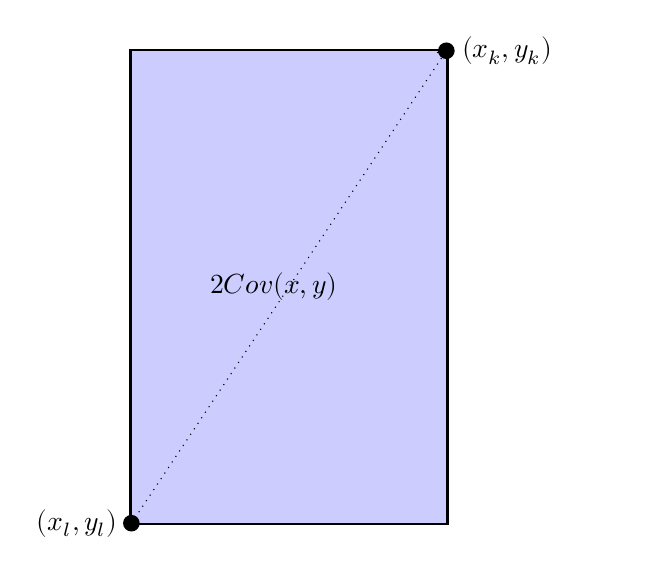
\begin{tikzpicture}
\draw  [-,ultra thick](0,0) -- (4,0) -- (4,6) -- (0,6) -- (0,0);
%\node[text width=2cm] at (3,-0.5){$\sqrt{2}~\sigma_x$};
%\node[text width=2cm] at (5.5,3){$\beta\sqrt{2}~\sigma_x$};
\filldraw[draw=black,fill=blue!20] (0,0) rectangle (4,6);
\draw[->,dotted] (0,0)--(4,6);
\node[text width=2cm] at (5.2,6){$(x_k,y_k)$};
\node[text width=2cm] at (-0.2,0){$(x_l,y_l)$};
\fill (4,6)  circle[radius=3pt];
\fill (0,0)  circle[radius=3pt];
\node[text width=2cm] at (2,3){$2Cov(x,y)$};
\end{tikzpicture}
\caption{Corr\'elation positive}
\end{figure}
 \end{leftcolumn}
  \begin{rightcolumn} %{0.48\textwidth}
  \begin{figure}
    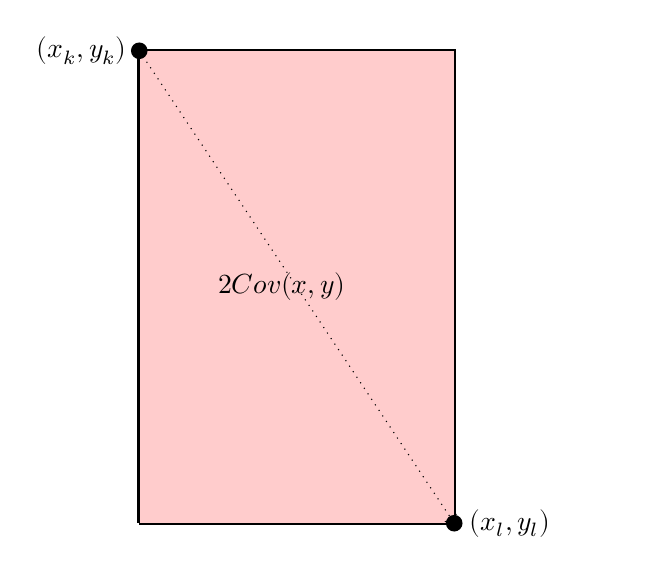
\begin{tikzpicture}
\draw [-,ultra thick](0,0) -- (4,0) -- (4,6) -- (0,6) -- (0,0);
%\node[text width=2cm] at (3,-0.5){$\sqrt{2}~\sigma_x$};
%\node[text width=2cm] at (5.5,3){$\beta\sqrt{2}~\sigma_x$};
\filldraw[draw=black,fill=red!20] (0,0) rectangle (4,6);
\draw[->,dotted] (0,6)--(4,0);
\node[text width=2cm] at (-0.3,6){$(x_k,y_k)$};
\node[text width=2cm] at (5.2,0){$(x_l,y_l)$};
%\draw (0,6) node[left] {$(x_k,y_k)$};
%\draw (6,0) node[left] {$(x_l,y_l)$};
\fill (0,6)  circle[radius=3pt];
\fill (4,0)  circle[radius=3pt];
\node[text width=2cm] at (2,3){$2Cov(x,y)$};
\end{tikzpicture}
\caption{Corr\'elation n\'egative}
\end{figure}
    \end{rightcolumn}
\end{paracol}

On a sample of N pairs of observations \((x_i,y_i)~i=1,\dots, N\) the empirical covariance can also be computed as the average of the \(N(N-1)\) areas of the \((x_i,y_i)\) and \((x_j,y_j)\) vertex rectangles for \(i=1,\dots, N-1\) and \(j=1,\dots, N\)
Note that the \(N\) rectangles (degenerate, of zero area) of vertex \((x_i,y_i)\) and \((x_j,y_j)\) with \(i=j\) should not be taken into account in the calculation.
\[Cov(x,~y)=\frac{1}{N(N-1)}\sum_{i=1}^{N-1} \sum_{j=i+1}^{N}~(x_i-x_j)(y_i-y_j)\]

An equivalent definition is to consider half (due to symmetry) of the average of the \(N(N-1)\) areas of the rectangles of vertices \((x_i,y_i)\) and \((x_j,y_j)\) for \(i=1,\dots, N\) and \(j=1,\dots, N\) (evidence in annexes).

\[Cov(x,~y)=\frac{1}{2N(N-1)}
\sum_{i=1}^{N} \sum_{j=1}^{N}~(x_i-x_j)(y_i-y_j)\]

\hypertarget{correlation}{%
\chapter{Correlation}\label{correlation}}

\hypertarget{from-covariance-to-correlation}{%
\section{from covariance to correlation}\label{from-covariance-to-correlation}}

The normalized version of the covariance, the correlation coefficient, however, shows by its magnitude the strength of the linear relation.

\begin{itemize}
\tightlist
\item
  Both covariance and correlation measure the relationship and the dependency between two variables.
\item
  Covariance indicates the direction of the linear relationship between variables.
\item
  Correlation measures both the strength and direction of the linear relationship between two variables.
\item
  Correlation values are standardized.
\item
  Covariance values are not standardized.
\end{itemize}

The normalized form of the covariance matrix is the correlation matrix.

\hypertarget{correlation-definition}{%
\section{Correlation definition}\label{correlation-definition}}

In statistics, correlation or dependence is any statistical relationship, whether causal or not, between two random variables or bivariate data.

In the broadest sense correlation is any statistical association, though it actually refers to the degree to which a pair of variables are linearly related.

There are several correlation coefficients, often denoted \(\rho\) or \(r\), measuring the degree of correlation. The most common of these is the Pearson correlation coefficient, which is sensitive only to a linear relationship between two variables (which may be present even when one variable is a nonlinear function of the other). Other correlation coefficients -- such as Spearman's rank correlation -- have been developed to be more robust than Pearson's, that is, more sensitive to nonlinear relationships.

\hypertarget{galton-a-pioneer-in-the-history-of-correlation}{%
\section{Galton, a pioneer in the history of correlation}\label{galton-a-pioneer-in-the-history-of-correlation}}

\begin{quote}
\begin{quote}
``I can only say that there is a vast field of topics that fall under the laws of correlation, which lies quite open to the research of any competent person who cares to investigate it.'' (Galton, 1890)
\end{quote}
\end{quote}

Galton's 1888 paper, presented to the Royal Society in London, defines correlation as follows:
\textgreater\textgreater{}``Two variable organs are said to be co-related when the variation of the one is accompanied on the average by more or less variation of the other, and in the same direction\ldots. It is easy to see that co-relation must be the consequence of the variations of the two organs being partly due to common causes\ldots{} If they were in no respect due to common causes, the co-relation would be nil.''

Galton's definition reveals the properties of the correlation coefficient. It is a measure of the strength of a linear relationship; the closer it is to 1, the more two variables can be predicted from each other by a linear equation. It is a measure of direction: a positive correlation indicates that \(X\), \(Y\) increase together; a negative correlation indicates that one decreases as the other increases. Note that Galton does not claim that co-relation implies cause and effect (it would be absurd to assume that the size of one organ determines the size of another). Galton hypothesized that the correlation indicated the presence of ``common causes'' for the observed relationship between the variables (the size of each organ respectively).

More technically Galton continues his presentation as follows:

\begin{quote}
\begin{quote}
``Let y = the deviation of the subject {[}in units of the probably error, Q{]}, whichever of the two variables may be taken in that capacity; and let x1, x2, x3, \&c., be the corresponding deviations of the relative, and let the mean of these be X. Then we find: (1) that y = rX for all values of y; (2) that r is the same, whichever of the two variables is taken for the subject; (3) that r is always less that 1; (4) that r measures the closeness of co-relation.''
\end{quote}
\end{quote}

Galton particularly liked the correlation coefficient because it could be used to predict deviations \(Y\) from \(X\) or \(X\) from \(Y\). Thus, from the beginning, the correlation coefficient was closely related to the regression line. Originally, \(r\) meant the regression slope, but there was a problem in that the regression line of the slope was partly a function of the units of measurement chosen. Galton perceived the correlation coefficient as a unitless regression slope and appropriated the label \(r\).

\includegraphics{galton.PNG}

\hypertarget{thirteen-ways-to-see-correlation-13cor}{%
\section{\texorpdfstring{thirteen ways to see correlation \citep{13cor}}{thirteen ways to see correlation {[}@13cor{]}}}\label{thirteen-ways-to-see-correlation-13cor}}

\begin{quote}
In 1885, Sir Francis Galton first defined the term ``regression'' and completed the theory of bivariate correlation. A decade later, Karl Pearson developed the index that we still use to measure correlation, Pearson's r . Our article is written in recognition of the 100th anniversary of Galton's first discussion of regression and correlation.
\end{quote}

According Joseph Lee Rodgers and co article, Several ways to interpret the correlation:

\begin{itemize}
\tightlist
\item
  As standardized covariance
  \[r=\frac{cov(x,y)}{\sigma^2_x\sigma^2_y}\]
\item
  As standardized slope of regression line
  \[r=b_{Y.X}(\frac{\sigma^2_x}{\sigma^2_y})=b_{X.Y}(\frac{\sigma^2_y}{\sigma^2_x})\]
\item
  As geometric mean of the two regression slopes\}\textbackslash{}
  \[r=\pm\sqrt{b_{Y.X}\times b_{X.Y}}\]
\item
  As the square root of the ratio of two variances\}
  \[r=\sqrt{\frac{\sum(Y_i -\hat{Y}_i)}{\sum(Y_i -\bar{Y}_i)}}=\sqrt{\frac{SS_{reg}}{SS_{tot}}}\]
\item
  And so many other\ldots{}
\end{itemize}

\hypertarget{pearson-correlation-coefficient}{%
\section{Pearson correlation coefficient}\label{pearson-correlation-coefficient}}

\begin{itemize}
\tightlist
\item
  some notations that may be useful:
\end{itemize}

\(S_{xx} = \sum_{i=1}^n(x_i -\bar{x})^2\)

\(S_{yy} = \sum_{i=1}^n(y_i -\bar{y})^2\)

\(S_{xy} = \sum_{i=1}^n(x_i -\bar{x})(y_i -\bar{y})\)

\begin{itemize}
\tightlist
\item
  Pearson correlation coefficient:
\end{itemize}

\[\rho=\frac{S_{xy}}{\sqrt{S_{xx}S_{yy}}}\]

The Pearson correlation coefficient is a bounded index (i.e., \(-1 \leq \rho \leq 1\)) that provides a unitless measure for the strength and direction of the association between two variables.

\hypertarget{spearmans-rank-correlation-coefficient}{%
\section{Spearman's rank correlation coefficient}\label{spearmans-rank-correlation-coefficient}}

measures the association based on the ranks of the variables.

\[\hat{\theta}=\frac{\sum_{i=1}^n(R_i-\bar{R}(S_i-\bar{S}))}{\sqrt{\sum_{i=1}^n(R_i-\bar{R})^2\sum_{i=1}^n(S_i-\bar{S})^2}}\]

where \(R_i\) and \(S_i\) are the rank of the \(x_i\) and \(y_i\) values, respectively.

Note that this is just the estimated Pearson's correlation coeffcient, but the values of the variables have been replaced by their respective ranks.

The Spearman correlation is the non-parametric equivalent of the Pearson correlation. It measures the relationship between two variables. If the variables are ordinal, discrete or do not follow a normal distribution, the Spearman correlation is used. This correlation does not use the values of the data but their rank.
In fact, nothing changes, everything is the same as calculating a Pearson correlation but on transformed variables.
The interest of establishing a correlation on the ranks of the variables is to detect if there is a monotonic relationship, which may not be linear.

\hypertarget{partial-correlation}{%
\section{Partial Correlation}\label{partial-correlation}}

The partial correlation coefficient, noted here \(r_{AB.C}\), allows us to know the value of the correlation between two variables A and B, if the variable C had remained constant for the series of observations considered.

Put another way, the partial correlation coefficient \(r_{AB.C}\) is the total correlation coefficient between variables A and B when we have removed their best linear explanation in terms of C. It is given by the formula :

\[r_{AB.C}=\frac{r_{AB}-r_{AC} \cdot r_{BC}}{\sqrt{1-r_{AC}^2} \cdot \sqrt{1-r_{BC}^2}}\]
Let's go a little further in understanding this coefficient:

The OLS estimator of \(\beta\) is written
\[\hat{\beta}=\frac{Cov(y,x_1)}{\mathbb{V}ar(x_1)}\]
The estimator \(\beta'\) is written

\begin{align*}
\hat{\beta'} &= \frac{Cov(y,x_1)\mathbb{V}(x_2)-Cov(y,x_2)Cov(x_1,x_2)}{
\mathbb{V}(x_1)\mathbb{V}(x_2)-Cov(x_1,x_2)^2} \\
&= \hat{\beta'}=\frac{\rho_{y1} \sigma_y \sigma_1\sigma_2^2-\rho_{y2} \sigma_y \sigma_2\rho_{12} \sigma_1 \sigma_2}{\sigma_1^2\sigma_2^2-\rho_{12}^2 \sigma_1^2 \sigma_2^2} \\
&= \hat{\beta'}=\underbrace{\frac{\rho_{y1}-\rho_{y2}\rho_{12}} 
{1-\rho_{12}^2}}_{qu'\grave{e}saco ?}\quad\frac{\sigma_y}{\sigma_1}
\end{align*}

some transformation\ldots{}
\[\hat{\beta'}=\underbrace{\underbrace{\frac{\rho_{y1}-\rho_{y2}\rho_{12}} 
{\sqrt{1-\rho_{12}^2}\sqrt{1-\rho_{y2}^2}}}_{corr\acute{e}lation ~partielle}}_{\rho_{y1|2}}
\quad\frac{\sigma_y\sqrt{1-\rho_{y2}^2}}{\sigma_1\sqrt{1-\rho_{12}^2}}\]

why\ldots Consider the following two regressions:
\(x_1=\kappa +\tau x_2+\varepsilon_{1|2}\) et \(y=\delta +\gamma x_2+\varepsilon_{y|2}\)

We have:
\begin{align*}
Cov(e_{1|2},e_{y|2})&=Cov(x_1-\hat{\kappa}-\hat{\tau} x_2,~y-\hat{\delta} -\hat{\gamma} x_2)\\
&=Cov(x_1,y)-\hat{\gamma}Cov(x_1,x_2)-\hat{\tau}Cov(x_1,y)+\hat{\gamma}\hat{\tau}\mathbb{V}ar(x_2)\\
\mathbb{V}ar(e_{y|2})&=\mathbb{V}ar(y-\hat{\delta} - \hat{\gamma} x_2)\\
&=\mathbb{V}ar(y)-2\hat{\gamma}Cov(x_1,y)+\hat{\gamma}^2\mathbb{V}ar(x_2)\\
\mathbb{V}ar(e_{1|2})&=\mathbb{V}ar(x_1-\hat{\kappa} - \hat{\tau} x_2)\\
&=\mathbb{V}ar(x_1)-2\hat{\tau}Cov(x_1,x_2)+\hat{\tau}^2\mathbb{V}ar(x_2)
\end{align*}

The linear correlation coefficient between \(e_{1|2}\) and \(e_{y|2}\) corresponds to the correlation between \(y\) and \(x_1\) after taking into account the linear influence of \(x_2\) on these two respective variables:

\begin{align*}
\rho_{yx_1|x_2}&=\frac{Cov(e_{1|2},e_{y|2})}{\sqrt{\mathbb{V}ar(e_{y|2})\mathbb{V}ar(e_{1|2})}}\\
\end{align*}

After simplification we obtain the expression of the partial correlation:

\begin{align*}
\rho_{y1|2}&=\frac{\rho_{y1}-\rho_{y2}\rho_{12}}{\sqrt{(1-\rho_{y2}^2)(1-\rho_{12}^2)}}
\end{align*}

everything becomes clearer\ldots{}

The estimator \(\hat{\beta'}\) can thus be written as that of a simple linear regression where the variables are the residuals of prior regressions of \(y\) respectively \(x_1\) on \(x_2\).

\[\hat{\beta'}=\rho_{y1|2}\frac{\sigma_y\sqrt{1-\rho_{y2}^2}}{\sigma_1\sqrt{1-\rho_{12}^2}}\]

\hypertarget{semi-partial-correlation}{%
\section{Semi partial Correlation}\label{semi-partial-correlation}}

\begin{align*}
sp\rho_{y1|2}&=\frac{\rho_{y1}-\rho_{y2}\rho_{12}}{\sqrt{1-\rho_{12}^2}}
\end{align*}

\hypertarget{transitivity-correlation}{%
\section{Transitivity correlation}\label{transitivity-correlation}}

Let \(\rho_{xy}\) be the correlation between the variables \(X\) and \(Y\). Let \(\rho_{xz}\) and \(\rho_{yz}\) be the correlations of variables \(X\) and \(Y\) with respect to a third variable \(Z\).

Given \(\rho_{xz}\) and \(\rho_{yz}\), can we deduce the possible values for \(\rho_{xy}\)?

\(\rho_{XY \mid Z}={\frac {\rho_{XY}-\rho _{XZ}\rho_{YZ}}{{\sqrt {1-\rho_{XZ}^{2}}}{\sqrt {1-\rho_{YZ}^{2}}}}}\)

\begin{align*}
  \rho_{XY} 
  &=  \left( \rho_{XY \mid Z} - \frac{ - \rho_{XZ} \rho_{YZ}}{\sqrt{1 - \rho_{XZ}^{2}} \sqrt{1 - \rho_{YZ}^{2}}} \right)  \sqrt{1 - \rho_{XZ}^{2}} \sqrt{1 - \rho_{YZ}^{2}}  \\
  &=  \rho_{XY \mid Z} \sqrt{1 - \rho_{XZ}^{2}} \sqrt{1 - \rho_{YZ}^{2}} +  \rho_{XZ} \rho_{YZ}
\end{align*}

\(\rho_{xy}\) is in the range \(\rho_{XZ} \rho_{YZ} \pm \sqrt{1 - \rho_{XZ}^{2}} \sqrt{1 - \rho_{YZ}^{2}}\)

\begin{align*}
  \rho_{XZ} \rho_{YZ} - \sqrt{1 - \rho_{XZ}^{2}} \sqrt{1 - \rho_{YZ}^{2}} &> 0 \\
  \rho_{XZ} \rho_{YZ} + \sqrt{1 - \rho_{XZ}^{2}} \sqrt{1 - \rho_{YZ}^{2}} &> 0 .
\end{align*}

\begin{align*}
  \rho_{XZ}^2 \rho_{YZ}^2 
  &> \left ( 1 - \rho_{XZ}^{2}\right ) \left (1 - \rho_{YZ}^{2}\right ) \\
  &= 1 - \rho_{XZ}^{2} - \rho_{YZ}^{2} + \rho_{XZ}^2 \rho_{YZ}^2 .
\end{align*}
Si \(\rho_{xy}>0\) alors on a

\begin{align*}
  \rho_{XZ}^2 \rho_{YZ}^2 
  &> \left ( 1 - \rho_{XZ}^{2}\right ) \left (1 - \rho_{YZ}^{2}\right ) \\
  &= 1 - \rho_{XZ}^{2} - \rho_{YZ}^{2} + \rho_{XZ}^2 \rho_{YZ}^2 .
\end{align*}

\begin{equation*}
\text{sign}(\rho_{XY}) 
  =
\begin{cases}
    \text{sign}(\rho_{XZ}) \text{sign}(\rho_{YZ}) & \rho_{XZ}^2 + \rho_{YZ}^2 > 1  \\
    \text{not known} & \rho_{XZ}^2 + \rho_{YZ}^2 \leq 1.
  \end{cases}
\end{equation*}

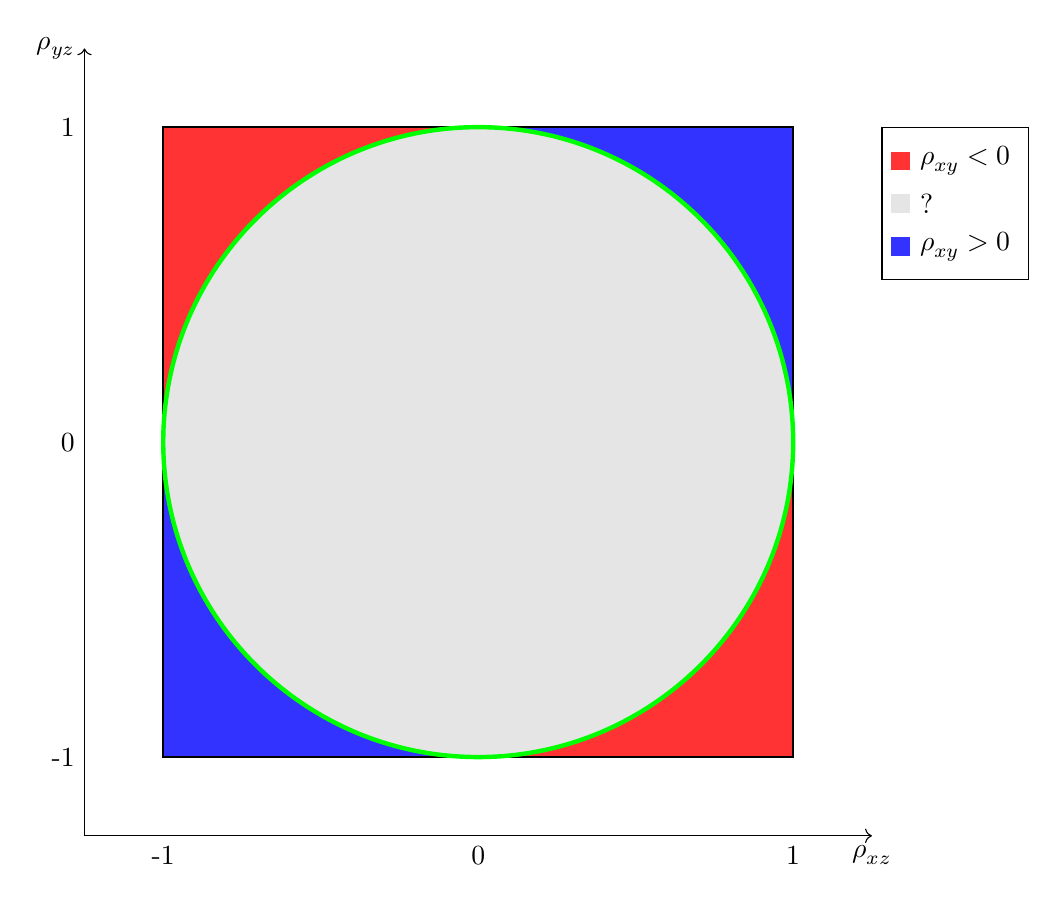
\begin{tikzpicture}
\draw [thick,fill=red!80] (0,4) rectangle (4,8);
\draw [thick,fill=red!80] (4,0) rectangle (8,4);
\draw [thick,fill=blue!80] (0,0) rectangle (4,4);
\draw [thick,fill=blue!80] (4,4) rectangle (8,8);
\draw[ultra thick,green,fill=gray!20] (4,4) circle (4cm);


\draw[->] (-1,-1) -- (9,-1) node[below] {$\rho_{xz}$} node[below] at(0,-1) {-1} node[below] at(4,-1) {0} node[below] at(8,-1) {1};
\draw[->] (-1,-1) -- (-1,9) node[left] {$\rho_{yz}$}
node[left] at(-1,0) {-1} node[left] at(-1,4) {0} node[left] at(-1,8) {1};

\matrix [draw,below left] at (11,8) {
  \node [rectangle,fill=red!80,label=right:$\rho_{xy}<0$] {};\\
  \node [rectangle,fill=gray!20,label=right:$?$] {};\\  
  \node [rectangle,fill=blue!80,label=right:$\rho_{xy}>0$] {};\\
};

%current bounding box.north east
\end{tikzpicture}

\hypertarget{distance-correlation}{%
\subsection{Distance correlation}\label{distance-correlation}}

The so-called association measures are an active and recent field of research that renews the well established and old field of correlation. The \emph{energy} package developed under R as well as Gabor's article \citep{discor} are good references.

Let \((x_i,y_i)\), \(i=1,2, \dots, N\) be a sample of pairs of observations of the variables \(X\) and \(Y\).

We compute successively

\[dx_{ij}=\lVert x_i-xj \rVert\]
\[dy_{ij}=\lVert y_i-yj \rVert\]

\[\overline{\overline{dx_{ij}}}=dx_{ij}-\overline{dx_{i.}}-\overline{dx_{.j}}+\overline{dx_{..}}\]
\[\overline{\overline{dy_{ij}}}=dy_{ij}-\overline{dy_{i.}}-\overline{dy_{.j}}+\overline{dy_{..}}\]
with

\(\overline{dx_{i.}}=\frac{1}{N}\sum_{j=1}^{N} dx_{ij}\)

and

\(\overline{dx_{..}}=\frac{1}{N^2}\sum_{i=1}^{N}\sum_{j=1}^{N} dx_{ij}\)

\[dCov(X,Y)=\frac{1}{N^2}\sum_{i=1}^{N}\sum_{j=1}^{N}
\overline{\overline{dx_{ij}}}~ 
\overline{\overline{dy_{ij}}}\]

\[dVar(X)=dCov^2(X,X)=\frac{1}{N^2}\sum_{i=1}^{N}\sum_{j=1}^{N} 
\overline{\overline{dx_{ij}}}~^2\]

\[d\rho=\frac{dCov(X,Y)}{d\sigma_X~d\sigma_Y}\]

\textbf{note bousquet : expliquer, commenter, représenter, tester sur un exmple, appliquer le package R, +bootstrap pour intervalles de confiance}

\hypertarget{other-correlations}{%
\section{Other Correlations}\label{other-correlations}}

\textbf{A développer si d'autre type de corrélation à rajouter}

\hypertarget{vizualization-of-covariance}{%
\chapter{Vizualization of covariance}\label{vizualization-of-covariance}}

\hypertarget{state-of-the-art-different-attempts-to-represent-the-covariance}{%
\section{State of the art: different attempts to represent the covariance}\label{state-of-the-art-different-attempts-to-represent-the-covariance}}

\hypertarget{diagramme-de-venn}{%
\subsection{diagramme de Venn}\label{diagramme-de-venn}}

\begin{quote}
A Venn diagram is a widely used diagram style that shows the logical relation between sets, popularized by John Venn in the 1880s. The diagrams are used to teach elementary set theory, and to illustrate simple set relationships in probability, logic, statistics, linguistics and computer science. A Venn diagram uses simple closed curves drawn on a plane to represent sets. Very often, these curves are circles or ellipses.
\end{quote}

\begin{figure}
    \centering
    \includegraphics[width= 250 pt]{venn_colinearity.PNG}
    \caption{Ballentine Venn diagrams displaying modest and considerable collinearity.}
    \label{fig:my_label}
\end{figure}

\hypertarget{visualizing-distributions-of-covariance-matrices}{%
\subsection{Visualizing Distributions of Covariance Matrices}\label{visualizing-distributions-of-covariance-matrices}}

\begin{quote}
\begin{quote}
Covariance matrices and their corresponding distributions play an important role in statistics. To understand the properties of distributions, we often rely on visualization methods. \citep{VisCov}
\end{quote}
\end{quote}

Visualizing a distribution in a high-dimensional space is a challenge, with the additional
difficulty that covariance matrices must be positive semi-definite, a restriction that forces
the joint distribution of the covariances into an oddly-shaped subregion of the space.

\includegraphics{wtf_covViz.PNG}

\hypertarget{a-geometrical-interpretation-of-an-alternative-formula-for-the-sample-covariance}{%
\subsection{A Geometrical Interpretation of an Alternative Formula for the Sample Covariance}\label{a-geometrical-interpretation-of-an-alternative-formula-for-the-sample-covariance}}

Kevin Hayes \citep{Hayes} proposes a new geometric and visual interpretation of covariance, based on the application of Hefferman's formula for variance. He extends this formula to the covariance of a sample to extract his results.

\begin{itemize}
\tightlist
\item
  formula from heffernan definition of covariance :
\end{itemize}

\[cov(X,Y)= \frac{2}{n(n-1)}\sum_{i=1}^{n-1}\sum_{j>i}^{n}\frac{1}{2}(x_i-x_j)(y_i - y_j)\]

\begin{quote}
\begin{quote}
Geometrically, \(\frac{1}{2}(x_i-x_j)(y_i - y_j)\) is ±1 times the area right-triangle formed with the difference vector \((x_i — x_j, y_j)\) as its hypotenuse, where negatively sloped difference tors incur a \((—1)\) sign and positively sloped difference vectors take a \((+1)\) sign. \citep{Hayes}
\end{quote}
\end{quote}

\includegraphics{hayes.PNG}

\hypertarget{covariance-as-signed-area-of-rectangles}{%
\subsection{Covariance as Signed Area of Rectangles}\label{covariance-as-signed-area-of-rectangles}}

This article \citep{chudzicki} was written following a very interesting conversation on the \textbf{stats.statckexchange} site. The initial topic of this conversation was: how to explain covariance to someone who only understands the notion of mean?

\textbf{instructions for use :}

\begin{itemize}
\tightlist
\item
  Draw all possible such rectangles. Color them transparently, making the positive rectangles red (say) and the negative rectangles ``anti-red'' (blue).
\item
  The covariance is the net amount of red in the plot (treating blue as negative values).
\end{itemize}

Let's deduce some properties of covariance. Understanding of these properties will be accessible to anyone who has actually drawn a few of the rectangles. :

\begin{itemize}
\tightlist
\item
  Bilinearity.
\end{itemize}

Because the amount of red depends on the size of the plot, covariance is directly proportional to the scale on the x-axis and to the scale on the y-axis.

\begin{itemize}
\tightlist
\item
  Correlation.
\end{itemize}

Covariance increases as the points approximate an upward sloping line and decreases as the points approximate a downward sloping line. This is because in the former case most of the rectangles are positive and in the latter case, most are negative.

\begin{itemize}
\tightlist
\item
  Relationship to linear associations.
\end{itemize}

Because non-linear associations can create mixtures of positive and negative rectangles, they lead to unpredictable (and not very useful) covariances. Linear associations can be fully interpreted by means of the preceding two characterizations.

\begin{itemize}
\tightlist
\item
  Sensitivity to outliers.
\end{itemize}

A geometric outlier (one point standing away from the mass) will create many large rectangles in association with all the other points. It alone can create a net positive or negative amount of red in the overall picture.

\includegraphics{covRect.PNG}

\hypertarget{our-current-project-the-package-plotnetrec}{%
\section{Our current project: the package plotnetrec}\label{our-current-project-the-package-plotnetrec}}

\hypertarget{plotnetrec}{%
\subsection{Plotnetrec}\label{plotnetrec}}

\includegraphics{All.PNG}

\hypertarget{hetrogeneity}{%
\subsection{Hetrogeneity}\label{hetrogeneity}}

\begin{minipage}{0.45\textwidth}
\centering
  \includegraphics{graph_plotnetrec_normal.png}
\end{minipage} 
\hspace{3.5ex}
\begin{minipage}{0.45\textwidth}
\centering
    \includegraphics{plot_rect_normal.png}
\end{minipage}
\begin{minipage}{0.45\textwidth}
\centering
    \includegraphics{graph_plotnetrec_heterogene.png}
\end{minipage} 
\hspace{3.5ex}
\begin{minipage}{0.45\textwidth}
\centering
    \includegraphics{graph_rect_heterogene.png}
\end{minipage}

\hypertarget{heterosdasticity}{%
\subsection{Heterosdasticity}\label{heterosdasticity}}

\begin{minipage}{0.45\textwidth}
    \includegraphics{graph_plotnetrec_normal.png}
\end{minipage} 
\hspace{3.5ex}
\begin{minipage}{0.45\textwidth}
    \includegraphics{plot_rect_normal.png}
\end{minipage}
\begin{minipage}{0.45\textwidth}
    \includegraphics{graph_plotnetrect_heterosk.png}
\end{minipage} 
\hspace{3.5ex}
\begin{minipage}{0.45\textwidth}
    \includegraphics{graph_rect_heterosk.png}
\end{minipage}

\hypertarget{non-linear-relationship}{%
\subsection{Non linear relationship}\label{non-linear-relationship}}

\begin{minipage}{0.45\textwidth}
    \includegraphics{graph_plotnetrec_normal.png}
\end{minipage} 
\hspace{3ex}
\begin{minipage}{0.45\textwidth}
    \includegraphics{graph_plotnetrect_nolinear.png}
\end{minipage}

\hypertarget{linear-regression-and-first-reliability-measure}{%
\chapter{Linear regression and first reliability measure}\label{linear-regression-and-first-reliability-measure}}

\hypertarget{ols-two-variables}{%
\section{OLS two variables}\label{ols-two-variables}}

\hypertarget{simple-linear-regression-model}{%
\subsection{simple linear regression model}\label{simple-linear-regression-model}}

\[y_i = \beta_0 + \beta_1x_i +  \epsilon_i\]
where \(\epsilon_i\) is te error or deviation of \(y_i\) from the line \(\beta_0 + \beta_1x_i\)

\begin{itemize}
\tightlist
\item
  Ordinary least square
\end{itemize}

We need to find the values of \(\beta_0\) and \(\beta_1\) that minimize the criterion :
\[S = \sum_{i=1}^n \epsilon_i^2 = \sum_{i=1}^n (y_i - (\beta_0 + \beta_1x_i))^2\]

Minimize this sum gives :

\[\hat{\beta_0}= \bar{y} - \hat{\beta_1}\bar{x}\]
\[\hat{\beta_1}= \frac{\sum_{i=1}^n(x_i -\bar{x})(y_i -\bar{y})}{\sum_{i=1}^n(x_i -\bar{x})^2}\]

\begin{itemize}
\tightlist
\item
  estimated simple linear regression model :
\end{itemize}

\[y_i = \hat{\beta_0} + \hat{\beta_1x_i} +  e_i\]

from which we can calculate a few additionnal quantities :

\begin{itemize}
\item
  \(\hat{y_i} = \hat{\beta_0} + \hat{\beta_1x_i}\) ; \(\hat{y_i}\) is the \textbf{predicted value} (or predicted fit) of y for the \(i^{th}\) observation in the sample.
\item
  \(e_i=y_i -\hat{y_i}\) ; is the \textbf{observed error} (or residual) for the \(i^{th}\) observation in the sample.
\item
  \(SSE = \sum_{i=1}^n (y_i -\hat{y_i})^2\) ; is the \textbf{sum of squared observed errors} for all observations in a sample of size \(n\)
\end{itemize}

\hypertarget{measuring-overall-variation-from-the-sample-line}{%
\subsection{Measuring overall variation from the sample line}\label{measuring-overall-variation-from-the-sample-line}}

\begin{itemize}
\item
  \(MSE = \frac{SSE}{n-p}\) , where \(p\) is the number of parametrers of the regression equation. \(p=2\) for regression with only one variable.
\item
  \(s = RMSE = \sqrt{(MSE)}\)
\item
  \(SSTO=\sum_{i=1}^n (y_i -\bar{y_i})^2\)
\item
  coefficient of determination :
\end{itemize}

\(R^2 = \frac{SSTO-SSE}{SSTO} = \frac{SSR}{SSTO}\) is the proportion of variation in \(y\) that is explained by \(x\).

i.e.~the coefficient of determination is then the ratio of the variance explained by the SSE regression to the total SST variance.

The coefficient of determination is the square of the linear correlation coefficient R between the predicted values \(\hat{y}_{i}\) and the measurements \(y_i\):

\[R^2=corr(\hat{y}_{i},y_i)\]

\(R^2\) does not indicate whether:

\begin{itemize}
\tightlist
\item
  the independent variables are a cause of the changes in the dependent variable;
\item
  omitted-variable bias exists;
\item
  the correct regression was used;
\item
  the most appropriate set of independent variables has been chosen;
\item
  there is collinearity present in the data on the explanatory variables;
\item
  the model might be improved by using transformed versions of the existing set of independent variables;
\item
  there are enough data points to make a solid conclusion.
\end{itemize}

\hypertarget{ols-plus-de-deux-variables}{%
\section{OLS plus de deux variables}\label{ols-plus-de-deux-variables}}

\textbf{A remplir ou A enlever}

\hypertarget{vizualisation-of-regression-and-correlation-beetween-variable}{%
\chapter{Vizualisation of regression and correlation beetween variable}\label{vizualisation-of-regression-and-correlation-beetween-variable}}

\hypertarget{state-of-the-art-1}{%
\section{State of the art}\label{state-of-the-art-1}}

\hypertarget{more-on-venn-diagrams-for-regression-figure-6.1}{%
\subsection{More on Venn Diagrams for Regression (figure 6.1)}\label{more-on-venn-diagrams-for-regression-figure-6.1}}

Kennedy \citep{kennedy} extended the Venn diagram to the exposition of bias and variance in the context of the classical linear regression (CLR) model, written as y = Xb + e .

\begin{itemize}
\tightlist
\item
  Purple area: variation in y uniquely explained by variation in X
\item
  A larger purple area means that more information is used in estimation, implying a smaller variance of the \(\beta_x\) estimate.
\item
  The black area: the variation in y that cannot be explained by X
\end{itemize}

\begin{figure}
    \centering
    \includegraphics[width= 250 pt]{vennken.PNG}
    \caption{Venn Diagram}
\end{figure}

\textbf{Another example of venn diagram: Relating species richness to the structure of continuous landscapes}

\begin{itemize}
\tightlist
\item
  Venn diagram representing the partition of the variance of the response variable Y (species richness) between two sets of explanatory variables, namely landscape data (a) and space (c).
\item
  The variance jointly explained by landscape data and space is represented by (b) in the diagram. The rectangle represents the total variance in Y (figure 6.2).
\end{itemize}

\begin{figure}
    \centering
    \includegraphics[width= 250 pt]{venn.PNG}
    \caption{Venn Diagram}
\end{figure}

\hypertarget{a-geometric-approach-to-compare-variables-in-a-regression-model}{%
\subsection{A Geometric Approach to Compare Variables in a Regression Model}\label{a-geometric-approach-to-compare-variables-in-a-regression-model}}

He proposes \citep{Bring} a geometric approaches to compare variables in a regression model.

\begin{quote}
This article gives a brief introduction to the geometric approach in regres- sion analysis, and then geometry is used to shed some light on the problem of comparing the ``importance'' of the in- dependent variables in a multiple regression model. Even though no final answer of how to assess variable impor- tance is given, it is still useful to illustrate the different measures geometrically to gain a better understanding of their properties.
\end{quote}

The model vector, \(\hat{y}\) is the perpendicular projection of y on x. Why it is the best estimate?

\begin{itemize}
\tightlist
\item
  The squared length of y, \(||y||^2 = \sum y_i^2\) is the total sum of square, \(SS_{tot}\)
\item
  The square length of \(\hat{y}\), \(||\hat{y}||^2= \sum \hat{y}^2=SS_{reg}\)
\item
  The square length of the vector \(y-\hat{y}\), \(||y - \hat{y}||^2=\sum(y_i-\hat{y}_i)^2 = SS_{res}\)
\end{itemize}

In other words, the observations vector is decomposed into a model vector and an error vector, and the shortest possible length of \(y-\hat{y}\) is found by projecting y perpendicular in x.

\begin{itemize}
\tightlist
\item
  The shortest possible length of \(y - \hat{y}\) is found by projecting \(y\) perpendicular on \(x\).
\item
  \(R^2 = \frac{SS_{reg}}{SS_{tot}}= \frac{||\hat{y}||^2}{||y||^2}\) (the \(y\) vector is standardized to have lenght 1.)
\item
  \[r_{xy} = 
  \begin{cases} ||\hat{y}||  \ \ \ \text{if}  \  \theta \leq 90 \degree \ \ \ \text{or} \ \theta \geq 270 \degree  \\ -||\hat{y}|| \ \ \ \text{if}  \ 90\degree \leq \theta \leq 270\degree
  \end{cases}\]
\end{itemize}

\begin{figure}
    \centering
    \includegraphics[width= 250 pt]{bring1.PNG}
    \caption{A remplir}
\end{figure}

\begin{figure}
    \centering
    \includegraphics[width= 250 pt]{bring.PNG}
    \caption{A remplir}
\end{figure}

\hypertarget{two-additional-views-of-linear-regression-coefficients}{%
\subsection{Two Additional Views of Linear Regression Coefficients}\label{two-additional-views-of-linear-regression-coefficients}}

The author \citep{Cli} proposes an interesting interpretation of the slope in the keast square method. The linear regression line of y on x, as determined by the method of least squares, passes through the central point with slope.

\textbf{A View of Linear Regression Coefficients as a weighted average slope}

\begin{itemize}
\tightlist
\item
  Consider any point \(P_i=(x_i,y_i)\) and \(P_o=(\bar{x}, \bar{y})\), the slope of the line \(P_i P_o\) is : \(b_i=\frac{y_i -\bar{y}}{x_i-\bar{x}}\)
\item
  Let's attach a weight \(w_i\) to each \(b_i\), if 2 points are very close, their slope is not very reliable (need little weight)
\item
  The ``distance'' between two points \(\to\) the distance projected on the x-axis. To avoid negative weight, we may then take the weight, \(w_i=(x_i-\bar{x})^2\)
\item
  Adopting this system of weighting, we see that b is the weighted mean of the \(b_i\)'s.
  \begin{equation}
                    b=\bar{b}=\frac{\sum b_i w_i}{\sum w_i} = \hat{\beta_1} = \frac{\sum(x_i -\bar{x})(y_i -\bar{y})}{\sum(x_i -\bar{x})^2}
                \end{equation}
\end{itemize}

\begin{quote}
This concept of weight for a slope is represented in the accompanying diagrams. (See Figure 1). The slope in the lefthand side diagram has a much larger weight than that in the righthand side for regression of y on x. If we were concerned with the regression of x on y, the reverse would be true. Note that the actual distance between the two points in the two diagrams is the same.
\end{quote}

\begin{figure}
    \centering
    \includegraphics[width= 250 pt]{LI_slope.PNG}
    \caption{A remplir}
\end{figure}

\hypertarget{our-current-project-the-plotnetrec-package}{%
\section{Our current project, the plotnetrec package:}\label{our-current-project-the-plotnetrec-package}}

\hypertarget{ols-diagramatic-representation}{%
\subsection{OLS Diagramatic representation}\label{ols-diagramatic-representation}}

The principle of construction of the following diagram giving a diagrammatic representation of the regression and OLS is :

\begin{itemize}
\tightlist
\item
  we assume that the covariance (an average of all possible rectangles as seen previously among all pairs of points in a data sample) can be represented by a rectangle.
\item
  This rectangle has by definition a known area given by the calculation of the empirical covariance \(Cov(X,Y)\). But the covariance depends on three parameters since \(Cov(X,Y) =\rho \sigma_x \sigma_y\) . To represent the covariance and draw the corresponding
  the corresponding rectangle, we have to make an additional assumption i.e.~choose a normalization \footnote{see appendix for a complement}.
  We assume that one side of this rectangle is normalized by \(sigma_x\). In this case, the other side necessarily has a length of \(\rho \sigma_y\).
\item
  Following the same approach, we now assume that the variances of \(X\) and \(Y\) can be represented by two squares whose sides are of course the standard deviations of \(X\) and \(Y\) respectively.
\end{itemize}

The diagram allows:

\begin{itemize}
\tightlist
\item
  to represent the OLS estimator by the slope of the diagonal of the rectangle representing the covariance. Geometrically, we obtain that if \(X\) increases by one standard deviation then \(Y\) increases by \(\rho\) standard deviation of the dependent variable Y.
\item
  to represent the explained variance in the total variance.
\item
  Correctly represent the coefficient of determination as the relative share of the explained variance in the total variance. With Venn diagrams sometimes used to represent the \(R^2\), visual perception is based on the relative size of two surfaces and their intersection. The proposed diagram is not an ad hoc construction, it is based on a methodological and theoretical foundation allowing not only to represent the \(R^2\) but also to read its value correctly.
\end{itemize}

reminder:

\begin{align*}
& \rho = \frac{COV(X,Y)}{\sigma_x \sigma_y}\\
\Leftrightarrow & COV(X,Y) = \rho \sigma_y \times \sigma_x
\end{align*}

\hypertarget{diagrammatic-representation}{%
\subsubsection{Diagrammatic representation}\label{diagrammatic-representation}}

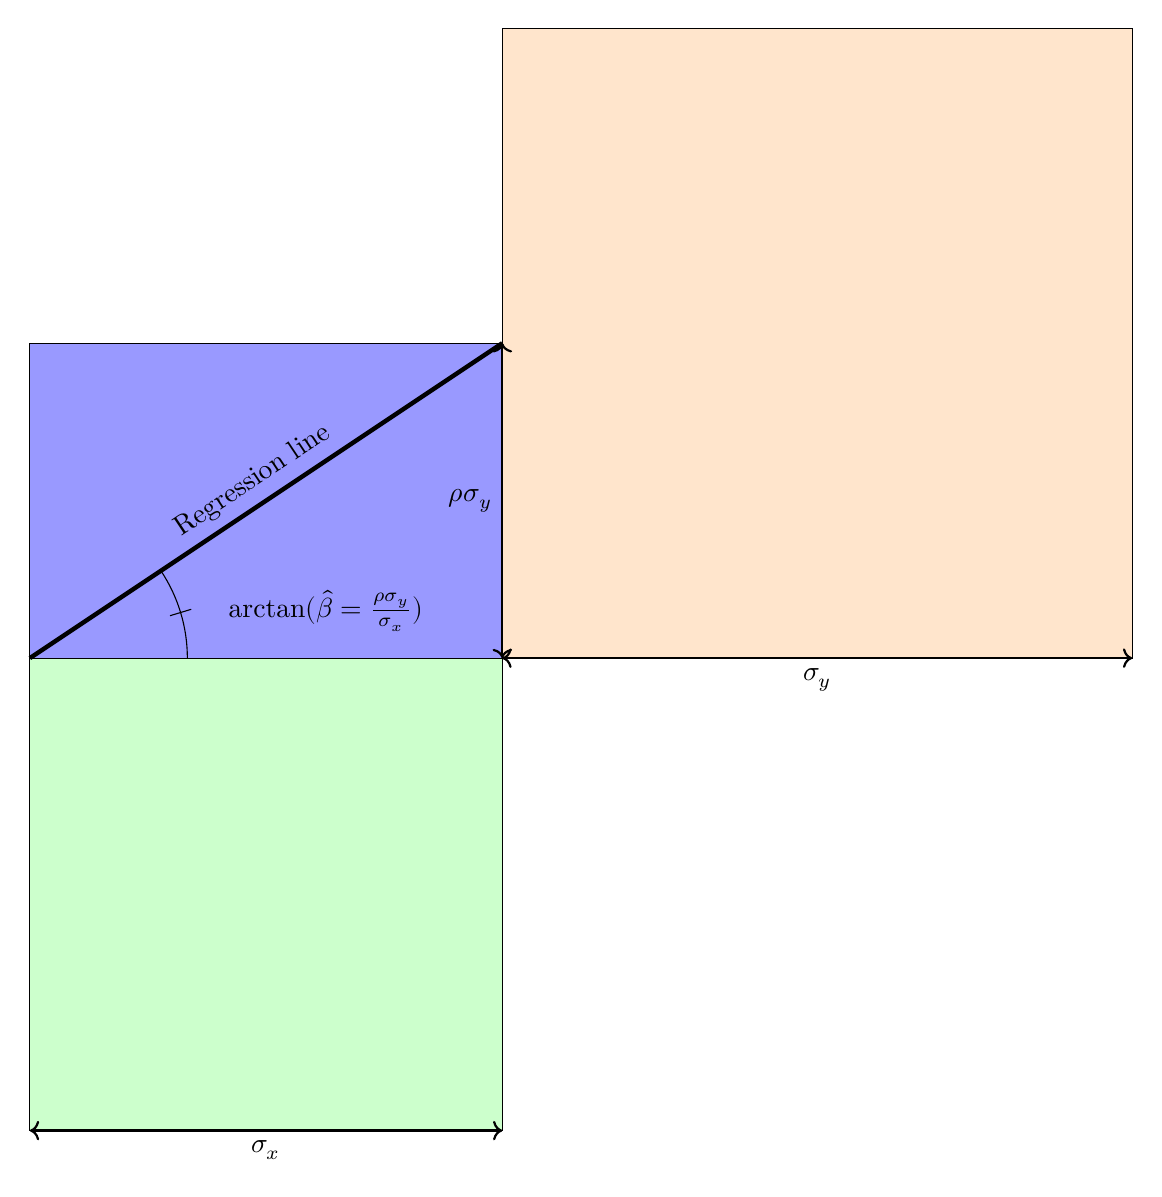
\begin{tikzpicture} [scale=2]
\def\sx{3};
\def\sy{4};
\def\r{0.5}; %postive%
\coordinate (O) at (0,0);
\coordinate (A) at (-\sx,-\sx);
\coordinate (B) at (\sy,\sy);
\coordinate (C) at (-\sx,{\sy*\r});
\draw[fill=green!20!white, draw=black] (O) rectangle (A); %variance for X%
\draw[fill=orange!20!white, draw=black] (O)rectangle (B); %variance for Y%
\draw[<->,fill=blue!40!white, draw=black] (O)rectangle(C);%covariance%
\draw[<->,thick] (A) -- node[below] {$\sigma_x$} (0,-\sx);
\draw[<->,thick] (O) -- node[below] {$\sigma_y$} (\sy,0);
\draw[<->,thick] (O) -- node[left] {$\rho\sigma_y$} (0,\r*\sy);


% draw angle for regression line%

%\pic [draw, ->, angle eccentricity=1.5] {angle = (0,0)--(-\sx,0)--(0,\r*\sy)};
%\draw[fill=green!30] (-\sx,0) -- (0,0) arc (0,\r*\sy);
%\tkzMarkAngle[size=1, draw=gray, arrows=->,arrowMe=stealth](P,O,M)]

\tkzDefPoint(0,0){t}
\tkzDefPoint(-\sx,0){tt}
\tkzDefPoint(0,\r*\sy){ttt}
\tkzMarkAngle[size=1, draw=black,fill=blue!20,mark=|](t,tt,ttt)]
\node[right] at (-\sx*0.6,0.3) {$\arctan( \hat{\beta}=\frac{\rho\sigma_y}{\sigma_x})$};  
% Regression line
\draw[-,ultra thick] (-\sx,0) -- node[midway,sloped,above] {Regression line} (0,\r*\sy);
\end{tikzpicture}

\hypertarget{representing-the-r2}{%
\subsubsection{\texorpdfstring{Representing the \(R^2\)}{Representing the R\^{}2}}\label{representing-the-r2}}

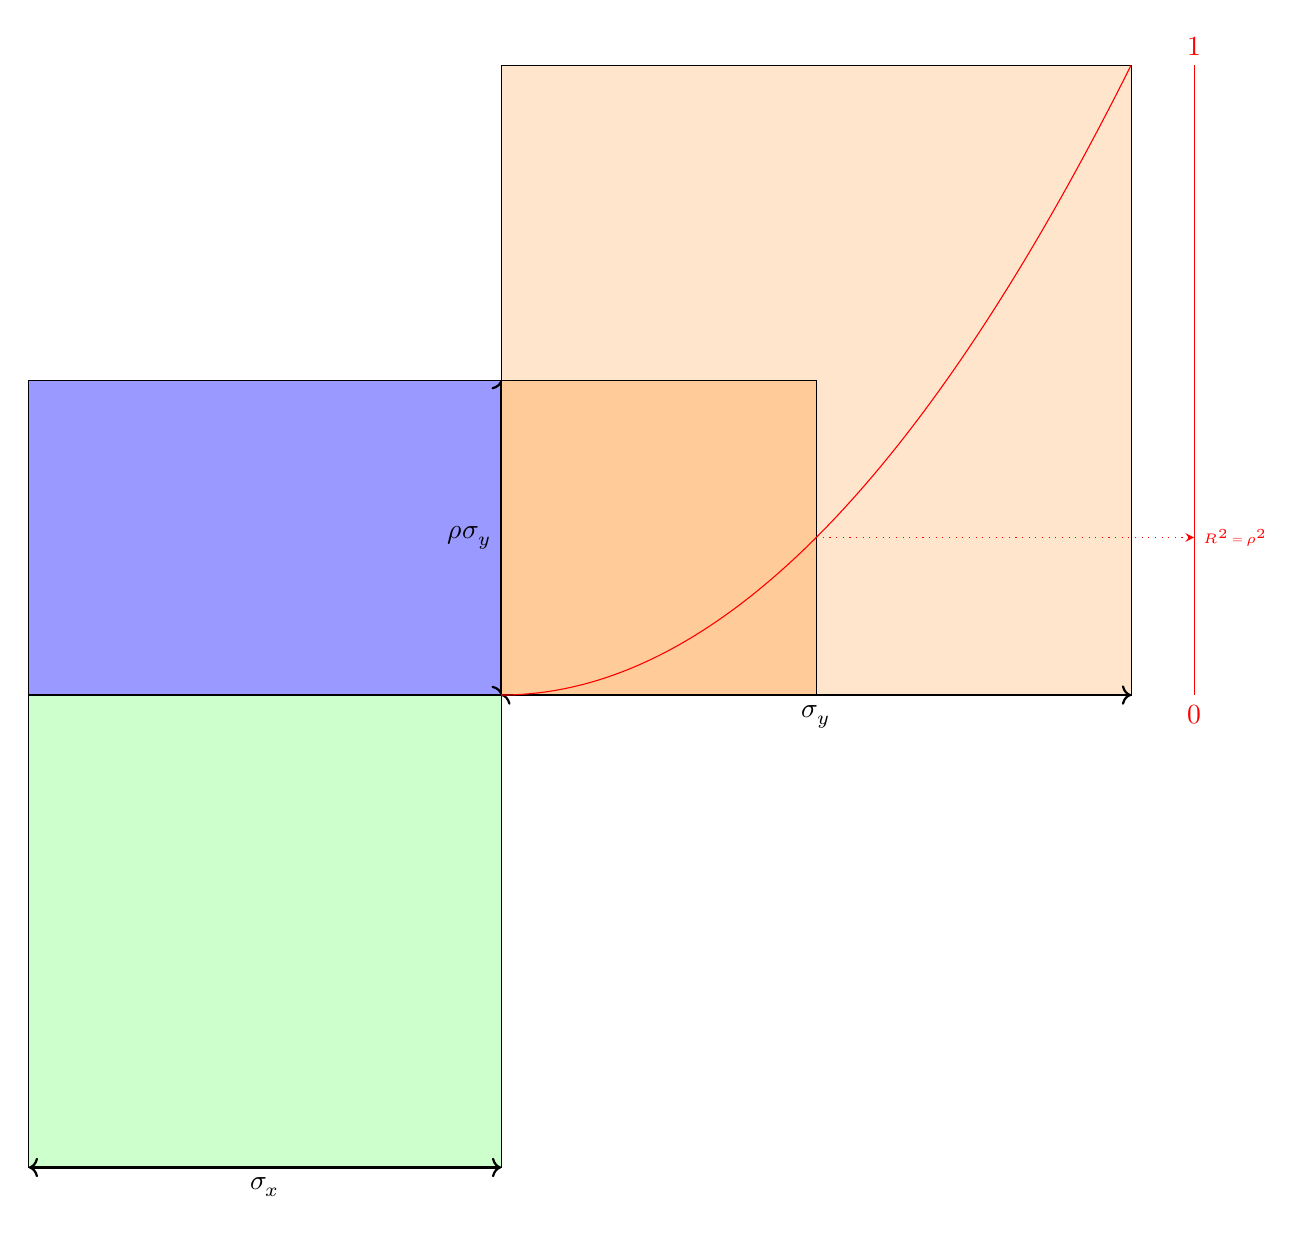
\begin{tikzpicture} [scale=2]
\def\sx{3};
\def\sy{4};
\def\r{0.5}; %positive%
\coordinate (O) at (0,0);
\coordinate (A) at (-\sx,-\sx);
\coordinate (B) at (\sy,\sy);
\coordinate (C) at (-\sx,{\sy*\r});
\draw[fill=green!20!white, draw=black] (O) rectangle (A); %variance for X%
\draw[fill=orange!20!white, draw=black] (O)rectangle (B); %variance for Y%
\draw[<->,fill=blue!40!white, draw=black] (O)rectangle(C);%covariance%
\draw[<->,thick] (A) -- node[below] {$\sigma_x$} (0,-\sx);
\draw[<->,thick] (O) -- node[below] {$\sigma_y$} (\sy,0);
\draw[<->,thick] (O) -- node[left] {$\rho\sigma_y$} (0,\r*\sy);

%exlained variance%
\draw[fill=orange!40!white, draw=black] (O)rectangle (\r*\sy,\r*\sy); 

% function r^2%
\draw[red,name path=curve 1,samples=200] plot[variable=\x,domain=0:\sy]
({\x},{(\x^2/\sy}); 

% read the value for R² and put a new scaled axe%
\draw [red] (\sy*1.1,0) node[below] {0} --(\sy*1.1,\sy) node [above] {1};
\draw [-stealth,dotted,red] (\r*\sy,\r^2*\sy) -- (\sy*1.1,\r^2*\sy) node[right,rotate=0]{\tiny $R^2=\rho^2$};

\end{tikzpicture}

\hypertarget{reg-lin-multiple}{%
\subsubsection{reg lin multiple}\label{reg-lin-multiple}}

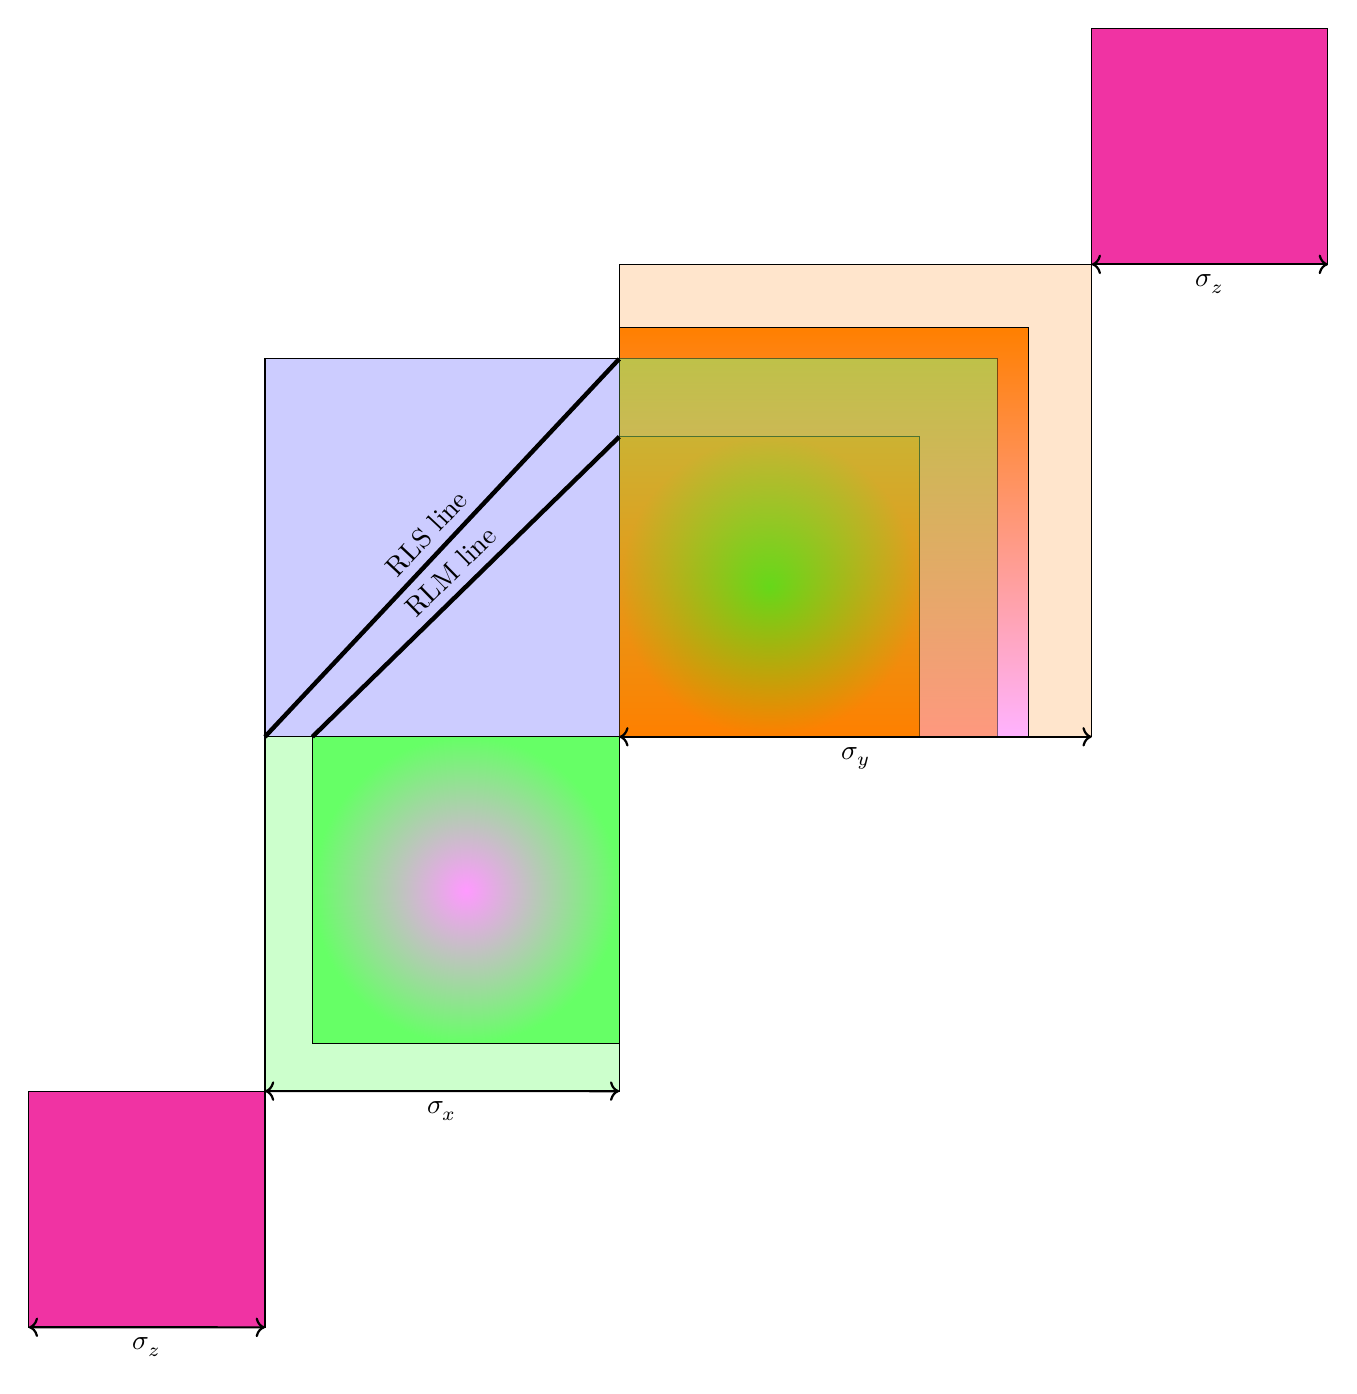
\begin{tikzpicture} [scale=1.5]
\def\sx{3};
\def\sy{4};
\def\sz{2}
\def\rxy{0.8}; %positive%
\def\rxz{0.5}; %positive%
\def\ryz{0.5}; %positive%
%$$$$$$$$$$$$$$$$$$$$$%
\def\vrxz{0.8660254}
\def\vryz{0.8660254}
\def\ryxz{0.7333333}I
%\def\truca{(sqrt(1-(\rxz)^2))};
%\def\truc{(-\sx*(sqrt(1-(\rxz)^2)))};
%\def\truc{-\sx*0.5};
\coordinate (O) at (0,0);
\coordinate (A) at (-\sx,-\sx);
\coordinate (B) at (\sy,\sy);
\coordinate (C) at (-\sx,{\sy*\rxy});
\coordinate (D) at (-\sx*\vrxz,-\sx*\vrxz);
\coordinate (E) at (\sy*\vryz,\sy*\vryz);
\coordinate (F) at (-\sx-\sz,-\sx-\sz);
\coordinate (G) at (\sy+\sz,\sy+\sz);
\coordinate (H) at (\ryxz*\vryz*\sy,\ryxz*\vryz*\sy);
\coordinate (I) at (\rxy*\sy,\rxy*\sy);

\draw[fill=magenta!80!white, draw=black] (A) rectangle (F); %variance for z%
\draw[fill=magenta!80!white, draw=black] (\sy,\sy) rectangle (G); %variance for z%

\draw[fill=green!20!white, draw=black] (O) rectangle (A); %variance for X%
\draw[fill=orange!20!white, draw=black] (O)rectangle (B); %variance for Y%
\draw[<->,fill=blue!20!white, draw=black] (O)rectangle(C);%covariance X Y%

%\draw[<->,thick] (O) -- node[left] {$\rho_{xy}\sigma_y$} (0,\rxy*\sy);

%\draw[fill=green!50!white, draw=black] (O) rectangle (D); %variance résiduelle x.z%
\shade[inner color=magenta!40, outer color=green!60,opacity=1, draw=black](O) rectangle (D); %variance résiduelle x.z%


%\draw[fill=orange!50!white, draw=black] (O) rectangle (E);%variance résiduelle y.z% 
\shade[top color=orange,bottom color=magenta!30,opacity=1,, draw=black] (O) rectangle (E);%variance résiduelle y.z% 
%\draw[fill=red!50!white, draw=black] (O) rectangle (H);%R2 partiel de X sur Y purgé de l'effet de Z% 
\shade[inner color=green,outer color=orange,draw=black] (O) rectangle (H);%R2 partiel de X sur Y purgé de l'effet de Z% 

%\draw[fill=gray!50!white, draw=black,opacity=0.5] (O) rectangle (I); %R2 RLS Y=a+bX%
\shade[top color=green!50,bottom color=orange,opacity=0.5, draw=black] (O) rectangle (I); %R2 RLS Y=a+bX%

\draw[<->,thick] (A) -- node[below] {$\sigma_x$} (0,-\sx);
\draw[<->,thick] (O) -- node[below] {$\sigma_y$} (\sy,0);
\draw[<->,thick] (F) -- node[below] {$\sigma_z$} (-\sx,-\sx-\sz);
\draw[<->,thick] (\sy,\sy) -- node[below] {$\sigma_z$} (\sy+\sz,\sy);
% Regression line
\draw[-,ultra thick] (-\sx,0) -- node[midway,sloped,above] {RLS line} (0,\rxy*\sy);
\draw[-,ultra thick] (-\sx*\vrxz,0) -- node[midway,sloped,above] {RLM line} (0,\ryxz*\vryz*\sy);


\end{tikzpicture}

\hypertarget{correlation-representation}{%
\subsection{Correlation representation}\label{correlation-representation}}

Need some reminders:

\[\rho = \frac{COV(X,Y)}{\sigma_x \sigma_y}\]
\[V(X+Y) = V(X) + V(Y) + 2COV(X,Y)\]
- Limits: \(\rho = 1\)

When \(\rho = 1\) then \(COV(X,Y) = \sigma_x \sigma_y\) \textbackslash{}
By replacing, we found: \(V(X+Y) = V(X) + V(Y) + 2\sigma_x \sigma_y\)

\begin{figure}
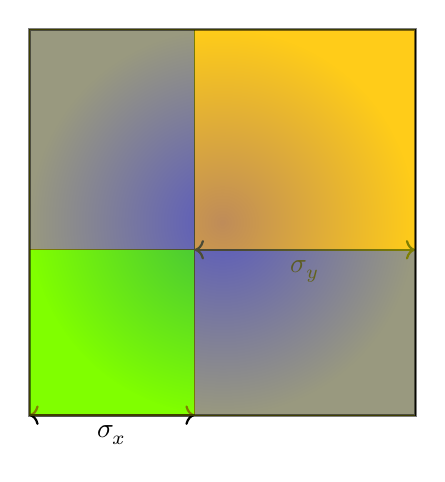
\begin{tikzpicture} [scale=0.7]
    \def\sx{3};
    \def\sy{4};
    \def\r{1}; %postive%
    \coordinate (O) at (0,0);
    \coordinate (A) at (-\sx,-\sx);
    \coordinate (B) at (\sy,\sy);
    \coordinate (C) at (-\sx,{\sy*\r});
    \draw[fill=green!580!white, draw=black] (O) rectangle (A); %variance for X%
    \draw[fill=orange!80!white, draw=black] (O)rectangle (B); %variance for Y%
        
  \draw[<->,fill=blue!80!white, draw=black] (O)rectangle(C);%covariance%
  \draw[<->,fill=blue!80!white, draw=black] (O)rectangle(\sy,-\sx);%covariance%
  
  \draw[<->,thick] (A) -- node[below] {$\sigma_x$} (0,-\sx);
  \draw[<->,thick] (O) -- node[below] {$\sigma_y$} (\sy,0);
  
  \shade[left color=green,outer color=yellow,opacity=0.5,draw=black,very thick](-\sx,-\sx) -- (-\sx,\sy) -- (\sy,\sy) -- (\sy,-\sx)-- cycle;
\end{tikzpicture}
\end{figure}

\begin{itemize}
\tightlist
\item
  Limits : \(\rho = -1\)
\end{itemize}

When \(\rho = -1\) then \(COV(X,Y) = -\sigma_x \sigma_y\) \textbackslash{}
By replacing, we found: \(V(X+Y) = V(X) + V(Y) - 2\sigma_x \sigma_y\)

\begin{figure}
    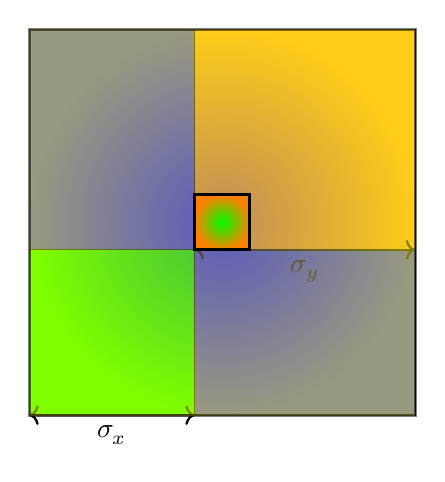
\begin{tikzpicture} [scale=0.7]
        \def\sx{3};
        \def\sy{4};
        \def\r{1}; %postive%
        \coordinate (O) at (0,0);
        \coordinate (A) at (-\sx,-\sx);
        \coordinate (B) at (\sy,\sy);
        \coordinate (C) at (-\sx,{\sy*\r});
        \draw[fill=green!580!white, draw=black] (O) rectangle (A); %variance for X%
        \draw[fill=orange!80!white, draw=black] (O)rectangle (B); %variance for Y%
        
  \draw[<->,fill=blue!80!white, draw=black] (O)rectangle(C);%covariance%
  \draw[<->,fill=blue!80!white, draw=black] (O)rectangle(\sy,-\sx);%covariance%
  
  \draw[<->,thick] (A) -- node[below] {$\sigma_x$} (0,-\sx);
  \draw[<->,thick] (O) -- node[below] {$\sigma_y$} (\sy,0);
        
  \shade[left color=green,outer color=yellow,opacity=0.5,draw=black,very thick](-\sx,-\sx) -- (-\sx,\sy) -- (\sy,\sy) -- (\sy,-\sx)-- cycle;
  \shade[inner color=green,outer color=orange,opacity=3.5,draw=black,very thick] (0,0) -- (0,\sy-\sx) -- (\sy-\sx,\sy-\sx) -- (\sy-\sx,0)-- cycle;
\end{tikzpicture}
\end{figure}

\begin{itemize}
\tightlist
\item
  Limits: \(\rho = 0\)
\end{itemize}

When \(\rho = 0\) then \(COV(X,Y) = 0\) \textbackslash{}
By replacing, we found: : \(V(X+Y) = V(X) + V(Y)\)

\begin{figure}
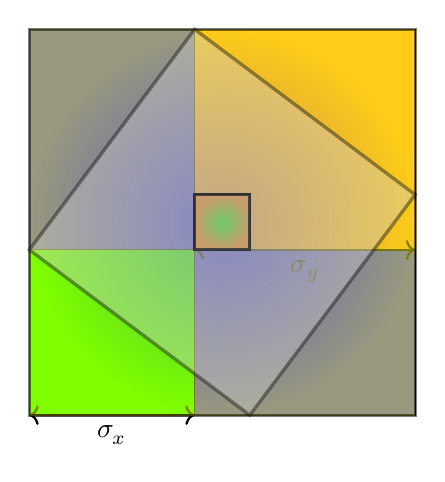
\begin{tikzpicture} [scale=0.7]
  \def\sx{3};
  \def\sy{4};
  \def\r{1}; %postive%
  \coordinate (O) at (0,0);
  \coordinate (A) at (-\sx,-\sx);
  \coordinate (B) at (\sy,\sy);
  \coordinate (C) at (-\sx,{\sy*\r});
  \draw[fill=green!580!white, draw=black] (O) rectangle (A); %variance for X%
  \draw[fill=orange!80!white, draw=black] (O)rectangle (B); %variance for Y%
  
  \draw[<->,fill=blue!80!white, draw=black] (O)rectangle(C);%covariance%
  \draw[<->,fill=blue!80!white, draw=black] (O)rectangle(\sy,-\sx);%covariance%
  
  \draw[<->,thick] (A) -- node[below] {$\sigma_x$} (0,-\sx);
  \draw[<->,thick] (O) -- node[below] {$\sigma_y$} (\sy,0);
  
  \shade[left color=green,outer color=yellow,opacity=0.5,draw=black,very thick](-\sx,-\sx) -- (-\sx,\sy) -- (\sy,\sy) -- (\sy,-\sx)-- cycle;
  \shade[inner color=green,outer color=orange,opacity=3.5,draw=black,very thick] (0,0) -- (0,\sy-\sx) -- (\sy-\sx,\sy-\sx) -- (\sy-\sx,0)-- cycle;
  
  \draw [<->,fill=gray!40!white, opacity=0.4,draw=black,very thick] (-\sx,0) -- (0,\sy) -- (\sy,\sy-\sx) -- (\sy-\sx,-\sx)-- cycle;
  \draw [<->,fill=gray!80!white, opacity=0.4,draw=black,very thick] (0,0) -- (0,\sy-\sx) -- (\sy-\sx,\sy-\sx) -- (\sy-\sx,0)-- cycle;
\end{tikzpicture}
\end{figure}

\textbackslash end\{frame\}

\begin{itemize}
\tightlist
\item
  Interest
\end{itemize}

Correlation matrix with distinct mathematical construction

\begin{figure}
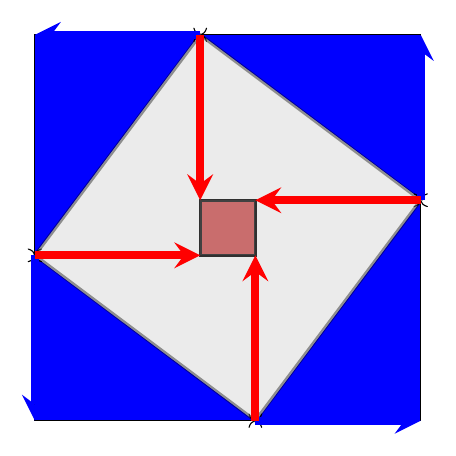
\begin{tikzpicture} [scale=0.7]
  \def\sx{3};
  \def\sy{4};
  \def\r{1}; %postive%
  \coordinate (O) at (0,0);
  \coordinate (A) at (-\sx,-\sx);
  \coordinate (B) at (\sy,\sy);
  \coordinate (C) at (-\sx,{\sy*\r});
  \draw[<->,fill=blue, draw=black] (-\sx,0) -- (-\sx,\sy) --(0,\sy);
  \draw[<->,fill=blue, draw=black] (-\sx,0) -- (-\sx,-\sx) --(\sy-\sx,-\sx);
  \draw[<->,fill=blue, draw=black] (\sy-\sx,-\sx) -- (\sy,-\sx) --(\sy,\sy-\sx);
  \draw[<->,fill=blue, draw=black] (0,\sy)--(\sy,\sy) --(\sy,\sy-\sx);
  
  \shade[top color=red,bottom color=red,opacity=3.5,draw=black,very thick] (0,0) -- (0,\sy-\sx) -- (\sy-\sx,\sy-\sx) -- (\sy-\sx,0)-- cycle;
  \draw [<->,fill=gray!40!white, opacity=0.4,draw=black,very thick] (-\sx,0) -- (0,\sy) -- (\sy,\sy-\sx) -- (\sy-\sx,-\sx)-- cycle;
  \draw [<->,fill=gray!80!white, opacity=0.4,draw=black,very thick] (0,0) -- (0,\sy-\sx) -- (\sy-\sx,\sy-\sx) -- (\sy-\sx,0)-- cycle;
  
  \draw [-stealth, color = blue,line width=3pt](0,\sy) -- (-\sx,\sy);
  \draw [-stealth,color = blue,  line width=3pt](-\sx,0) -- (-\sx,-\sx);
  \draw [-stealth,color = blue, line width=3pt](\sy-\sx,-\sx) -- (\sy,-\sx);
  \draw [-stealth,color = blue, line width=3pt](\sy,\sy-\sx) -- (\sy,\sy);
  
  \draw [-stealth, color = red, line width=3pt](0,\sy) -- (0,\sy - \sx);
  \draw [-stealth,color = red, line width=3pt](-\sx,0) -- (0, 0);
  \draw [-stealth,color = red, line width=3pt](\sy-\sx,-\sx) -- (\sy-\sx,0);
  \draw [-stealth,color = red, line width=3pt](\sy,\sy-\sx) -- (\sy-\sx,\sy-\sx);
  
\end{tikzpicture}
\end{figure}

\hypertarget{causality}{%
\chapter{Causality}\label{causality}}

In the basic model \(y^=\alpha+\beta x+\varepsilon\) the OLS estimator \(\hat{\beta}\) is unbiased if \(x\) is independent of \(\varepsilon\). We cannot know a priori if this is the case and in any case not a posteriori at the end of the estimation since the residuals are by construction independent of \(X\). We can easily show that there is no unique solution in \(\hat{\beta}\) of the maximum likelihood when we increase the model by a free parameter representing the correlation between \(\varepsilon\) and \(x\).
The prediction \(\mathbb{E}(y~/x)=\hat{\beta}x\) is correct only if \(\mathbb{E}(\varepsilon~/x)=0\).
Otherwise \(\mathbb{E}(\varepsilon~/x)=0\) there is an endogeneity and \(\hat{\beta}\) is not an exact measure of the marginal effect of an exogenous variation of \(x\).
The main situations of endogeneity encountered and studied are related to the problems :

\begin{itemize}
\tightlist
\item
  Simultaneous causality
\item
  Omitted variables
\item
  Measurement errors on the variables
\item
  Selection bias
\item
  Poorly specified functional form
\end{itemize}

\hypertarget{the-main-cases}{%
\section{The main cases}\label{the-main-cases}}

\hypertarget{simultaneous-causality}{%
\subsection{Simultaneous causality}\label{simultaneous-causality}}

Is it enough to simply show by a diagram that regressing y on x and then x on y does not give the same result?
The answer is no, it is not enough!

\hypertarget{omitted-variables}{%
\subsection{Omitted variables}\label{omitted-variables}}

\ldots. Repeat the previous results in a simplified way to illustrate the effect of omitting a variable and present the conditions under which the omission of a variable leads to a bias on the model parameters.

\hypertarget{measurement-errors}{%
\subsection{Measurement errors}\label{measurement-errors}}

Let's consider the following RLS model

\[y^{\star}=\alpha+\beta x^{\star}+\varepsilon\]

We do not observe \(y^{\star}\) (but \(y=y^{\star}+v_y\)), nor \(x^{\star}\) (but \(x=x^{\star}+u_x\)).

Consider the following assumptions:

\(\mathbb{E}(u_x)=\mathbb{E}(v_y)=0\)

\(\mathbb{E}(y v_y)=\mathbb{E}(y u_x)=\mathbb{E}(x u_y)=\mathbb{E}(x v_x)=0\)

\(\mathbb{E}(\varepsilon u_y)=0\)

The measurement errors are of zero expectation, and independent of the variables and the error term.
Under these assumptions, for two randomly chosen points \(k\) \(l\), the covariance between \(X\) and \(Y\) does not change.

\[\mathbb{E}[(x_k-x_l)(y_k-y_l)]\]

\[\mathbb{E}[(x_k^{\star}+u_k-(x_l^{\star}+u_l))(y_k^{\star}+v_k-(y_l^{\star}+v_l))]\]

\[\mathbb{E}[(x_k^{\star}+u_k)(y_k^{\star}+v_k)] -\mathbb{E}[x_k^{\star}+u_k]\mathbb{E}[y_l^{\star}+v_l] -\mathbb{E}[x_l^{\star}+u_l]\mathbb{E}[y_k^{\star}+v_k]+ \mathbb{E}[(x_l^{\star}+u_l)(y_l^{\star}+v_l)]\]

\[2Cov(x^{\star},y^{\star})\]

Measurement errors are detrimental to accuracy but on average they do not affect the covariance. The only essential problem is therefore related to the correct estimation of the parameters, while the correlation between the dependent and independent variables does not change. On the other hand, one should not confuse the effect of \(x\) on \(y\) with the effect of the measurement error of \(x\) on \(y\) (which is zero).

\hypertarget{measurement-error-on-the-dependent-variable}{%
\section{Measurement error on the dependent variable}\label{measurement-error-on-the-dependent-variable}}

Let us consider a measurement error on the dependent variable \(y\), i.e.~let \(\sigma_v^2 > 0\) and \(\sigma_u^2 = 0\). The model becomes:
\[y=alpha+beta x + v+ \varepsilon\]
The measurement error on the dependent variable does not matter in the sense that it has no biasing effect on the estimated parameters of the model. In practice, it can be considered as contributing to the disturbance term of the model. It is obviously undesirable, as anything that increases the noise in the model will tend to make the regression estimates less accurate, but it has no impact in terms of bias in the estimates.

In this case, we do not make a diagram for a graphical proof because it is so obvious!

\hypertarget{measurement-error-on-the-independent-variable}{%
\section{Measurement error on the independent variable}\label{measurement-error-on-the-independent-variable}}

We consider the case where the measurement error is on the dependent variable \(x\), i.e.~Let \(sigma_v^2 =0\) and \(sigma_u^2 >0\).
The model becomes:
\[y=alpha+beta x -beta u + \varepsilon\]

In the regression of \(y\) on \(x\), the measurement error of \(x\) becomes part of the error in the regression equation related to the parameter \(\beta\), thus creating an endogeneity bias. The OLS estimator \(\hat{\beta}=\frac{Cov(x,y)}{Var(x)}\) is biased towards 0. The unbiased estimator is \(\beta=frac{Cov(x^\star ,y)}{Var(x^\star)}\).

Proof:

Since \(Cov(x^\star,y)=Cov(x,y)\), we have:
\[\frac{\hat{\beta}}{\beta}=\frac{Var(x^\star)}{Var(x)}=\frac{\sigma_x^{\star 2}}{\sigma_u^2+\sigma_x^{\star 2}} \implies plim~\hat{\beta}=\lambda \beta\]
with \(\lambda=\frac{\sigma_x^{\star 2}}{\sigma_u^2+\sigma_x^{\star 2}}\). Since \(0<lambda<1\) the coefficient \(\hat{\beta}\) is biased towards 0.
The bias depends on the level and the sign of \(\beta\):
\[plim~\hat{\beta}-\beta=\lambda \beta-\beta=-(1-\lambda)\beta=-\frac{\sigma_u^2}{\sigma_u^2+\sigma_x^{\star 2}}\beta\]
\#\#\# Diagram of the model with measurement error on the independent variable
The following figure illustrates the problem in a very simple way.

\begin{figure}
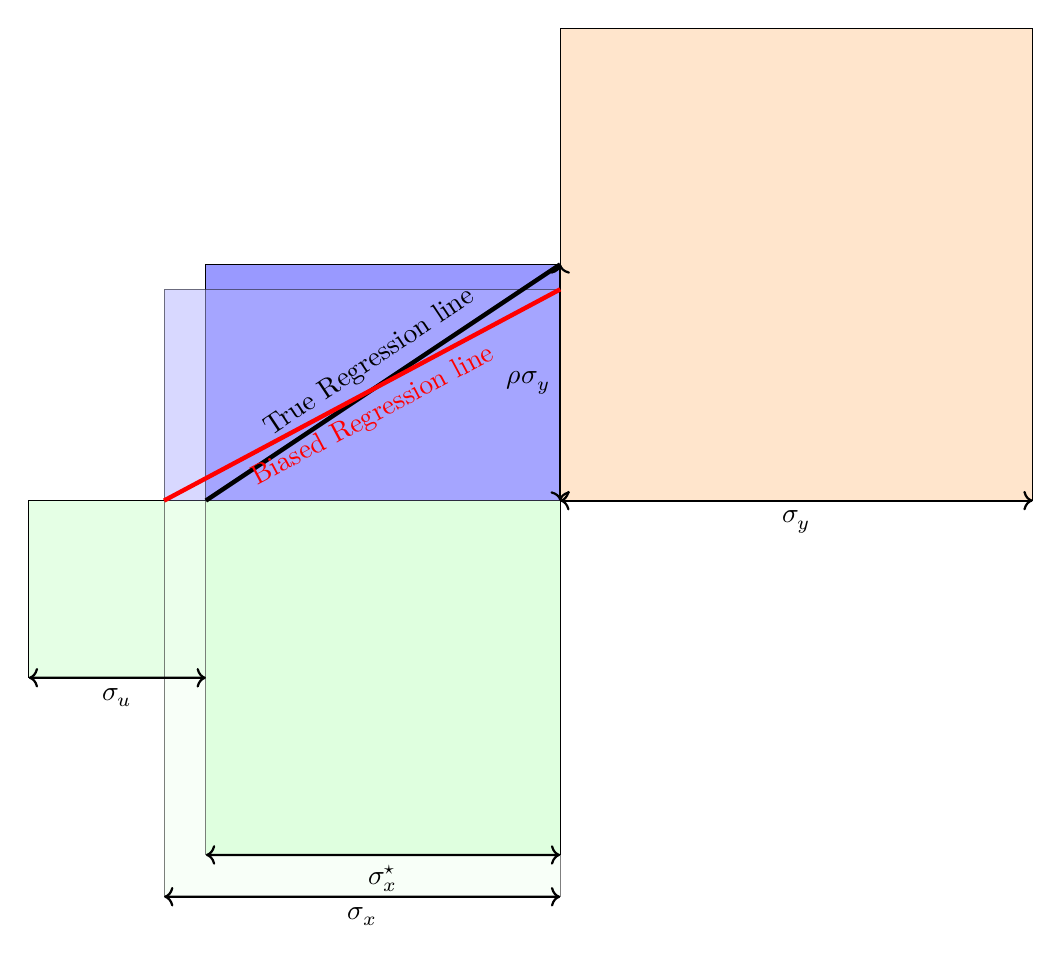
\begin{tikzpicture} [scale=1.5]
\def\sx{3};
\def\su{1.5};
\def\sxt{3.354101966};
\def\sy{4};
\def\r{0.5}; %positive%
\def\truc{1.788854382}
\coordinate (O) at (0,0);
\coordinate (A) at (-\sx,-\sx);
\coordinate (B) at (\sy,\sy);
\coordinate (C) at (-\sx,{\sy*\r});
\coordinate (D) at (-\sx,0);
\coordinate (E) at (-\sx-\su,-\su);
\coordinate (F) at (-\sxt,-\sxt);

\draw[fill=green!20!white, draw=black] (O) rectangle (A); %variance for X%
\draw[fill=orange!20!white, draw=black] (O)rectangle (B); %variance for Y%
\draw[<->,fill=blue!40!white, draw=black] (O)rectangle(C);%covariance%
\draw[<->,fill=green!10!white, draw=black] (D)rectangle(E);%variance for u%
\draw[fill=green!5!white, draw=black,opacity=0.5] (O) rectangle (F); %variance for Xt%
\draw[<->,fill=blue!30!white, draw=black,opacity=0.5] (-\sxt,0)rectangle(0,\truc);%covariance%

\draw[<->,thick] (A) -- node[below] {$\sigma_x^\star$} (0,-\sx);
\draw[<->,thick] (O) -- node[below] {$\sigma_y$} (\sy,0);
\draw[<->,thick] (O) -- node[left] {$\rho\sigma_y$} (0,\r*\sy);
\draw[<->,thick] (E) -- node[below] {$\sigma_u$} (-\sx,-\su);
\draw[<->,thick] (F) -- node[below] {$\sigma_x$} (0,-\sxt);
 
% Regression line
\draw[-,ultra thick] (-\sx,0) -- node[midway,sloped,above] {True Regression line} (0,\r*\sy);
% Biasied Regression line
\draw[-,ultra thick,red] (-\sxt,0) -- node[midway,sloped,below] {Biased Regression line} (0,\truc);
\end{tikzpicture}
\caption{\label{measurement error on x} Régression de $y$ sur $x$ avec erreur de mesure sur $x$}
\end{figure}

\hypertarget{instrumental-variables}{%
\section{Instrumental variables}\label{instrumental-variables}}

\[Y=\alpha + \beta X +u\]
\[X=\theta + \delta Z +v\]
\[\beta_{IV}=\frac{Cov(Y,Z)}{Cov(X,Z)} =\frac{\rho_{zy} \sigma_y}{\rho_{zx} \sigma_x}\]

\hypertarget{state-of-the-art-of-r-packages-in-visualization-econometrics-and-data-viz-more-broadly}{%
\chapter{State of the art of R packages in visualization econometrics (and data-viz more broadly)}\label{state-of-the-art-of-r-packages-in-visualization-econometrics-and-data-viz-more-broadly}}

\begin{itemize}
\tightlist
\item
  R energy
\end{itemize}

\textbf{A compléter}

\begin{itemize}
\tightlist
\item
  viscov
\end{itemize}

Our visualizations follow the principle of decomposing a covariance matrix into scale parameters and correlations, pulling out marginal summaries where possible and using two and three-dimensional plots to reveal multivariate structure. Visualizing a distribution of covariance matrices is a step beyond visualizing a single covariance matrix or a single multivariate dataset.

\begin{itemize}
\tightlist
\item
  Colourpicker
\end{itemize}

Colourpicker is a tool for Shiny framework and for selecting colours in plots. This tool supports various options, such as alpha opacity, custom colour palettes, and more. The most common uses of this tool include the utilisation of the colourInput() function to create a colour input in Shiny as well as the use of the plotHelper() function/RStudio Addin to select colours for a plot.

\begin{itemize}
\tightlist
\item
  Esquisse
\end{itemize}

The esquisse package allows a user to interactively explore data by visualising it with the ggplot2 package. It allows a user to draw bar graphs, curves, scatter plots, histograms, export the graphs, and retrieve the code generating the graph. With the help of esquisse, one can quickly visualise the data according to their type as well as export to PNG or PowerPoint, and retrieve the code to reproduce the chart.

\begin{itemize}
\tightlist
\item
  ggplot2
\end{itemize}

ggplot is a popular package that is based on the grammar of graphics. The idea behind this library is that one can build every graph from the same components, such as a dataset, a coordinate system, and more. The package provides graphics language for creating intuitive and intricate plots. It allows a user to create graphs that represent both univariate and multivariate numerical and categorical data.

\begin{itemize}
\tightlist
\item
  ggvis
\end{itemize}

ggvis is a data visualisation package for R that allows to declaratively describe data graphics with a syntax similar in spirit to ggplot2. It allows creating rich interactive graphics locally in Rstudio or in the browser as well as leverage the infrastructure of the Shiny package to publish interactive graphics usable from any browser. The goal of ggvis is to make it easy to build interactive graphics for exploratory data analysis.

\begin{itemize}
\tightlist
\item
  ggforce
\end{itemize}

The ggforce is a package aimed at providing missing functionality to ggplot2 through the extension system introduced with ggplot2 v2.0.0. The goal of this package is to provide a repository of geoms, stats, among others. Using ggforce, one can enhance almost any ggplot by highlighting data groupings and focusing attention on interesting features of the plot.

\begin{itemize}
\tightlist
\item
  lattice
\end{itemize}

Lattice is a powerful high-level data visualisation system for R that is designed with an emphasis on multivariate data and allows to create multiple small plots easily. The lattice package attempts to improve on base R graphics by providing better defaults and the ability to display multivariate relationships easily. Particularly, the package supports the creation of trellis graphs that show a variable or the relationship between variables, conditioned on one or more other variables.

\begin{itemize}
\tightlist
\item
  Plotly
\end{itemize}

Plotly is an open-source R package for creating interactive web-based graphs via the open-source JavaScript graphing library plotly.js. The Plotly's R graphing library helps in creating interactive, publication-quality graphs including line plots, scatter plots, area charts, bar charts, error bars, etc. One can use Plotly for R to make, view and distribute charts and maps online as well as offline.

\begin{itemize}
\tightlist
\item
  patchwork
\end{itemize}

patchwork is a package that expands the API to allow for the arbitrarily complex composition of plots by providing mathematical operators for combining multiple plots. The goal of patchwork is to make it simple to incorporate separate ggplots into the same graphic.

\begin{itemize}
\tightlist
\item
  quantmod
\end{itemize}

quantmod is an R package that provides a framework for quantitative financial modelling and trading. It provides a rapid prototyping environment that makes modelling easier by removing the repetitive workflow issues surrounding data management and visualisation.

\begin{itemize}
\tightlist
\item
  RGL
\end{itemize}

The RGL package is used to produce interactive 3-D plots using OpenGL. The library contains high-level graphics commands modelled loosely after classic R graphics and working in three dimensions. It also includes a low-level structure inspired by the grid package. RGL provides medium to high-level functions for 3D interactive graphics, including functions modelled on base graphics as well as functions for constructing representations of geometric objects.

\begin{itemize}
\tightlist
\item
  Highcharter
\end{itemize}

is an R wrapper for Highcharts, an interactive visualization library in JavaScript. Like its predecessor, highcharter features a powerful API.

Highcharter makes dynamic charting easy. It uses a single function, hchart(), to draw plots for all kinds of R object classes, from data frame to dendrogram to phylo. It also gives R coders a handy way to access the other popular Highcharts plot types, Highstock (for financial charting) and Highmaps (for schematic maps in web-based projects).

\begin{itemize}
\tightlist
\item
  Leaflet
\end{itemize}

Like highcharter, Leaflet for R is another charting packaged based on a hugely-popular JavaScript library of the same name.

Leaflet offers a lightweight but powerful way to build interactive maps, which you've probably seen in action (in their JS form) on sites ranging from The New York Times and The Washington Post to GitHub and GIS specialists like Mapbox and CartoDB.

The R interface for Leaflet was developed using the htmlwidgets framework, which makes it easy to control and integrate Leaflet maps right in R Markdown documents (v2), RStudio, or Shiny apps.

\begin{itemize}
\tightlist
\item
  RcolorBrewer
\end{itemize}

RColorBrewer makes it easy to take advantage of one of R's great strengths: manipulating colors in plots, graphs, and maps.

The package is based on Cynthia Brewer's work on the use of color in cartography (check out Colorbrewer to learn more), and it lets you create nice-looking sequential, diverging, or qualitative color palettes. It also plays nicely with Plotly, as these examples by Plotly demonstrate.

\begin{itemize}
\tightlist
\item
  dygraphs
\end{itemize}

This package provides an R interface for dygraphs, a fast, flexible JavaScript charting library for exploring time-series data sets. What's powerful about dygraphs is that it's interactive right out of the box, with default mouse-over labels, zooming, and panning. It's got lots of nifty other interactivity features, like synchronization or the range selector shown above.

But dygraph's interactivity doesn't come at the expense of speed: it can handle huge datasets with millions of points without slowing its roll. And you can use RColorBrewer with dygraphs to choose a different color palette for your time series--- check out this example to see how.

\begin{itemize}
\tightlist
\item
  sunburst
\end{itemize}

pas forcément utile pour notre sujet

\begin{itemize}
\tightlist
\item
  VennDiagram
\end{itemize}

Create a Venn diagram and save it into a file. The function venn.diagram() takes a list and creates a file containing a publication-quality Venn Diagram.

\hypertarget{annexes}{%
\chapter{annexes}\label{annexes}}

\hypertarget{correction-de-bessels-proof}{%
\section{Correction de Bessel's proof}\label{correction-de-bessels-proof}}

\begin{align*}
(n-1)S_{xy} &= \sum_{i=1}^{N}(x_i-\bar x)(y_i - \bar y) \\
&= \sum_{i=1}^{N} x_i y_i -N\bar x \bar y\\
&= \sum_{i=1}^{N} x_i y_i - \frac{1}{N}\sum_{i=1}^{N} x_i \sum_{i=1}^{N} y_i\\
(N-1) \mathbb{E}(S_{xy}) &= \mathbb{E}\left(\sum_{i=1}^{N} x_i y_i\right) 
- \frac{1}{N}\mathbb{E}\left(\sum_{i=1}^{N} x_i \sum_{i=1}^{N} y_i\right)\\
&= N\mu_{xy} - \frac{1}{N}[N\mu_{xy} + N(N-1)\mu_x \mu_y]\\ 
&= (N-1)[\mu_{xy}-\mu_x\mu_y]\\
&= (N-1)Cov(x,~y)
\end{align*}

\hypertarget{proof-for-covxyfrac12nn-1sum_i1n-sum_j1nx_i-x_jy_i-y_j}{%
\section{\texorpdfstring{Proof for \(Cov(x,~y)=\frac{1}{2N(N-1)}\sum_{i=1}^{N} \sum_{j=1}^{N}~(x_i-x_j)(y_i-y_j)\)}{Proof for Cov(x,\textasciitilde y)=\textbackslash frac\{1\}\{2N(N-1)\}\textbackslash sum\_\{i=1\}\^{}\{N\} \textbackslash sum\_\{j=1\}\^{}\{N\}\textasciitilde(x\_i-x\_j)(y\_i-y\_j)}}\label{proof-for-covxyfrac12nn-1sum_i1n-sum_j1nx_i-x_jy_i-y_j}}

\begin{itemize}
\tightlist
\item
  Proof 1
\end{itemize}

\[Cov(x,~y)=\frac{1}{2N(N-1)}
\sum_{i=1}^{N} \sum_{j=1}^{N}~(x_i-x_j)(y_i-y_j)
=\]

\[\frac{1}{2N(N-1)}
\sum_{i=1}^{N} N~x_i~y_i -x_i~N~\overline{y}-y_i~N~\overline{x}+N~\overline{xy}\]

\[\frac{2N^2}{2N(N-1)}(\overline{xy}-\overline{x}~\overline{y})=\]

\[\frac{N}{N-1}(\overline{xy}-\overline{x}~\overline{y}))\]

\begin{itemize}
\tightlist
\item
  Proof 2
\end{itemize}

another way, not uninteresting, to show the equivalence between the two formulations of the covariance but starting from the usual form.
\[Cov(x,~y)=\frac{1}{(N-1)}
\sum_{i=1}^{N} (x_i-\overline{x})(y_i -\overline{y})\]

\[Cov(x,~y)=\frac{1}{2(N-1)} \left\{
\sum_{i=1}^{N} (x_i-\overline{x})(y_i -\overline{y}) +
\sum_{j=1}^{N} (x_j-\overline{x})(y_j -\overline{y}) \right\}\]

\[Cov(x,~y)=\frac{1}{2N(N-1)} 
\sum_{i=1}^{N} \sum_{j=1}^{N}\left\{(x_i-\overline{x})(y_i -\overline{y}) + (x_j-\overline{x})(y_j -\overline{y}) \right\}\]

\[Cov(x,~y)=\frac{1}{2N(N-1)} 
\sum_{i=1}^{N} \sum_{j=1}^{N}\left\{(x_i-x_j)(y_i-y_j)+x_iy_j+x_jy_i-x_i\overline{y}-x_j\overline{y}-y_i\overline{x}-y_j\overline{x}+2~\overline{x}~\overline{y}\right\}\]

\[Cov(x,~y)=\frac{1}{2N(N-1)} 
\sum_{i=1}^{N} \sum_{j=1}^{N}\left\{(x_i-x_j)(y_i-y_j)\right\}\]

\hypertarget{a-little-bit-of-calculation}{%
\section{a little bit of calculation}\label{a-little-bit-of-calculation}}

\hypertarget{variance-of-the-sum-of-two-random-variables}{%
\subsubsection{Variance of the sum of two random variables}\label{variance-of-the-sum-of-two-random-variables}}

\begin{align*}
Var(X+Y) &= Cov(X+Y,X+Y)  \\
 &= E((X+Y)^2)-E(X+Y)E(X+Y)   \\
\text{en développant,}  \\
 &= E(X^2) - (E(X))^2 + E(Y^2) - (E(Y))^2 + 2(E(XY) - E(X)E(Y))  \\
 &= Var(X) + Var(Y) + 2(E(XY)) - E(X)E(Y))  \\
 &= Var(X) + Var(Y) + 2 Cov(X,~Y)  \\
\end{align*}

If the variables \(X,~Y\) are independent \(E(XY) = E(X)E(Y)\) then
\(Var(X+Y) = Var(X) + Var(Y)\)

\begin{align*}
\Delta &= 4Cov(X,~Y)^2-4Var(X)Var(Y)\\
&=4[Cov(X,~Y)^2-Var(X)Var(Y)] \leq 0\\
\end{align*}

So \$ Cov(X,Y)\^{}2 \leq Var(X) Var(Y)\$ (In probability theory, the Cauchy-Schwarz inequality allows the proof of the result because of the inequality \(E(XY)\leq \sqrt{E(X^2)E(Y^2)}\))
or \$-(X,Y) \leq \sigma\_x\sigma\_y \leq \sigma\_x\sigma\_y \$.
Let us notice that if \(\Delta=0\) then we have the equality \$ Cov(X,Y)\^{}2=Var(X) Var(Y)\$, i.e.~if there exists \(~\lambda\) such that \(Var(\lambda X+Y)=0\)\textbackslash{}
But to conclude, if we have \(~lambda X+Y\) equal with probability 1 to a constant, let's say \(c\), it is indeed that \(Y = c -~lambda X\) almost surely, in other words a perfect linear link between the two variables.

\hypertarget{definition-of-the-linear-correlation-coefficient-bravais-pearson}{%
\subsubsection{Definition of the linear correlation coefficient (Bravais-Pearson)}\label{definition-of-the-linear-correlation-coefficient-bravais-pearson}}

\begin{itemize}
\tightlist
\item
  case \(Cov(X,~Y)\geq 0\)
\end{itemize}

We define
\(\rho = \frac{2Cov(X,~Y)}{Var_{max}-Var_{min}}\)

\(Var_{max} = \sigma_X^2+\sigma_Y^2+2\sigma_X\sigma_Y\)

\(Var_{min} = \sigma_X^2+\sigma_Y^2\)

\(Var_{max}-Var_{minx} = 2\sigma_X\sigma_Y\)

from which, simplifying

\(\rho = \frac{Cov(X,~Y)}{\sigma_X\sigma_Y}\)

\begin{itemize}
\tightlist
\item
  case \(Cov(X,~Y)\leq 0\)
\end{itemize}

We define
\(\rho = \frac{2Cov(X,~Y)}{Var_{max}-Var_{min}}\)

\(Var_{max} = \sigma_X^2+\sigma_Y^2\)

\(Var_{min} = \sigma_X^2+\sigma_Y^2-2\sigma_X\sigma_Y\)

\(Var_{max}-Var_{minx} = 2\sigma_X\sigma_Y\)

from which, simplifying

\(\rho = \frac{Cov(X,~Y)}{\sigma_X\sigma_Y}\)

\hypertarget{covariance-framing}{%
\subsubsection{Covariance framing}\label{covariance-framing}}

\[-\sqrt{(Var(X)Var(Y)} \leq Cov(X,Y) \leq \sqrt{(Var(X)Var(Y)}\]

With in the particular case of standardized variables

\begin{align*}
Var(\frac{X}{\sigma_X}+\frac{Y}{\sigma_Y})&= Var(\frac{X}{\sigma_X})+Var(\frac{Y}{\sigma_Y})+2Cov(\frac{X}{\sigma_X},\frac{Y}{\sigma_Y})\\
&=2(1+\rho)\\
Var(\frac{X}{\sigma_X}-\frac{Y}{\sigma_Y})&= Var(\frac{X}{\sigma_X})+Var(\frac{Y}{\sigma_Y})-2Cov(\frac{X}{\sigma_X},\frac{Y}{\sigma_Y})\\
&=2(1-\rho)
\end{align*}
One finds, knowing that \(2(1+\rho) \geq 0\) and \(2(1-\rho)\geq 0\) that one has \(-1 \le \rho \le 1\)

\hypertarget{notes}{%
\chapter{Notes}\label{notes}}

\begin{itemize}
\tightlist
\item
  titre graphique; positionnement et taille graphique
\item
  reference aux graphiques et bibliographies
\item
  tout est ajoutable, déplacable, enlevable, modifiable. AUcun soucis
\item
  Bibliographie : parcourir doc et rajouter aticles oubliés dans bibliographie
\item
  position graphiques mal centrés ou mal dimensionné.
\item
  possibilité de mettre code R directement
\item
  Certaines parties vides: a remplir ou à mettre de coté pour l'instant ( on verra au second semestre)
\item
  rajouter plus d'applications R pour illustrer? plutot au second semestre je pense
\item
  prendre d'autres passages du beamer possible
\end{itemize}

  \bibliography{references.bib}

\end{document}
